\begin{acknowledgementsCH}
 這裡將簡單介紹如何利用\LaTeX\ 來編輯你的畢業論文,若不知道\LaTeX\ 是什麼或是沒有概念的話,建議你可以簡單看過放在此資料夾裡的\href{run:./latex123.pdf}{李果正-大家來學\LaTeX}前四章內容,在下載適合的\LaTeX\ 整合發行套件之後(請看第~\ref{it:download}項),可以嘗試用剛安裝好的\LaTeX\ 編輯器來編譯\href{run:./thesis.tex}{thesis.tex}這份文件,編譯的方法可以看下面第~\ref{it:comp}項的介紹,若編譯成功,所編譯出來的thesis.pdf文件的應該會跟此demo.pdf文件一模一樣,而且沒有任何問號符號,走到這一步的話,就差不多可以開始邊學習\LaTeX\ 邊編輯你的畢業論文了!基本上會使用到的指令都包含在論文的的各章節裡,怎麼在論文裡寫公式或是放圖之類的就自行看tex檔學吧。如果有任何問題或建議可以來信與我討論,我的信箱是\href{mailto:dran31545@gmail.com}{dran31545@gmail.com},或是到此範本\href{http://code.google.com/p/ntu-thesis-latex-template/}{Google Project}裡面的\href{http://code.google.com/p/ntu-thesis-latex-template/issues/list}{Issues}貼上你的問題與建議,我會盡我所能更新此範本,也歡迎大家自行重製、改良此範本並散布給他人,祝大家順利畢業!\\\\
 要編輯致謝請打開\href{run:./acknowledgementsCH.tex}{acknowledgementsCH.tex}\\
 \begin{enumerate}[leftmargin=0pt, topsep=0pt, itemsep=0pt, label=\Roman{*}.]
\item 此範本參考並修改自下列網站的資料:
\begin{enumerate}[topsep=0pt, itemsep=0pt, label=$\bullet$]
    \item \href{http://www.csie.ntu.edu.tw/~tzhuan/www/resources/ntu/}{如何用 LaTeX 排版臺灣大學碩士論文}\\
    \textemdash 台灣大學論文\LaTeX\ 樣版原創者\href{http://www.csie.ntu.edu.tw/~tzhuan/www/}{黃子桓}的教學網頁
    \item \href{http://www.hitripod.com/blog/2012/05/latex-thesis-template-quick-reference/}{LaTeX 常用語法及論文範本}\\
    \textemdash \href{http://www.hitripod.com/blog/}{Hitripod}所修改的範本,這裡參考了許多他所寫的格式和內容
    \item \href{http://www.cc.ntu.edu.tw/chinese/epaper/0014/20100920_1404.htm}{使用LaTeX做出精美的論文}
    \item \href{http://www.hitripod.com/blog/2011/04/xetex-chinese-font-cjk-latex/}{XeTeX:解決 LaTeX 惱人的中文字型問題}
    \item \href{http://code.google.com/p/ntuthesis/}{台灣大學碩士、博士論文的Latex模板}\\
\end{enumerate}
\item 幾個有用的參考資料及網路資源:
\begin{enumerate}[topsep=0pt, itemsep=0pt, label=$\bullet$]
    \item \href{run:./latex123.pdf}{李果正-大家來學\LaTeX}\textemdash 建議先看完前四章
    \item \href{http://en.wikibooks.org/wiki/LaTeX}{WIKIBOOKS-\LaTeX}\textemdash 好用的線上工具書
    \item \href{run:./Working_with_a_bib_file_using_Jabref.pdf}{Working with a .bib file using JabRef}
    \item \href{run:./Fi087_S.pdf}{Using BibDesk - A short tutorial}
    \item \href{http://www.dfcd.net/articles/latex/latex.html}{LaTeX for Physicists}\\
\end{enumerate}
\item 下載\LaTeX\ 整合發行套件,可參考\href{http://www.tug.org/texcollection/}{TeX Collection}:\label{it:download}
 \begin{enumerate}[topsep=0pt, itemsep=0pt, label=\arabic{*}.]
     \item \href{http://www.tug.org/mactex/}{MacTeX}: For \textcolor{Green}{\textbf{MacOSX}},下載\href{http://mirror.ctan.org/systems/mac/mactex/MacTeX.pkg}{MacTeX.pkg}
     \item \href{http://www.tug.org/protext/}{ProTeXt}: For \textcolor{Green}{\textbf{Windows}},下載\href{ftp://ftp.fernuni-hagen.de/pub/windows/win32/ProTeXt/}{ISO file}
     \item \href{http://www.tug.org/texlive/}{TeX Live}: For \textcolor{Green}{\textbf{GNU/Linux}} and \textcolor{Green}{\textbf{MacOSX}}, and \textcolor{Green}{\textbf{Windows}},下載\href{http://www.tug.org/texlive/acquire-iso.html}{ISO file}
     \item \href{http://ctan.org/}{CTAN}: The Comprehensive TeX Archive Network.\\
 \end{enumerate}

\item 好用的程式:
 \begin{enumerate}[topsep=0pt, itemsep=0pt, label=$\bullet$]
    \item 文獻管理系統:
        \begin{enumerate}[topsep=0pt, itemsep=0pt, label=\arabic{*}.]
         \item \href{http://jabref.sourceforge.net/}{JabRef}\\
                     可參考\href{run:./Working_with_a_bib_file_using_Jabref.pdf}{Working with a .bib file using JabRef}或是\href{https://www.google.com/search?q=jabref}{Google}及\href{http://www.youtube.com/results?search_query=jabref}{YouTube}
         \item \href{http://bibdesk.sourceforge.net/}{BibDesk} (For Mac)\\
                     可參考\href{run:./Fi087_S.pdf}{Using BibDesk - A short tutorial}或是\href{https://www.google.com/search?q=bibdesk}{Google}及\href{http://www.youtube.com/results?search_query=bibdesk}{YouTube}
         \end{enumerate}
         \item 方程式編輯器:\href{https://chrome.google.com/webstore/detail/dinfmiceliiomokeofbocegmacmagjhe?hl=zh-TW}{Daum Equation Editor} (Chrome App,必須使用Google瀏覽器)\\
 \end{enumerate} 
\item 編譯流程:\label{it:comp}
\begin{enumerate}[topsep=0pt, itemsep=0pt, label=\arabic{*}.]
    \item \texttt{xelatex thesis}\\ 對thesis.tex進行第一次XeLaTeX編譯,產生thesis.pdf以其他檔案
    \item \texttt{bibtex thesis}\\ 對thesis.tex進行BibTeX編譯,產生bbl檔以及blg檔
    \item \texttt{xelatex thesis}\\ 對thesis.tex進行第二次XeLaTeX編譯,產生目錄、圖表連結及參考文獻
    \item \texttt{xelatex thesis}\\ 對thesis.tex進行第三次XeLaTeX編譯,產生參考文獻連結,完成編譯
\end{enumerate} 
    \textcolor{Red}{注意!}此範本使用cite套件,可依據你利用文獻管理系統所整理好的\href{run:./thesisbib.bib}{thesisbib.bib}檔在論文最後產生參考文獻頁面,若你的系所規定要在每個章節的後面產生參考文獻,則可以用chapterbib套件,來對每個有附參考文獻的章節tex檔進行一次BibTeX編譯產生bbl檔,如範例的\href{run:./introduction.tex}{introduction.tex}、\href{run:./THM.tex}{THM.tex}和\href{run:./EXP.tex}{EXP.tex},如果有這需要請把\href{run:./thesis.tex}{thesis.tex}檔裡使用cite套件的指令利用註解符號\texttt{\%}來取消使用cite套件,並刪去出現在使用chapterbib套件指令前面的註解符號\texttt{\%}來啟動使用chapterbib套件
    \begin{verbatim}
\usepackage{cite}
%\usepackage{chapterbib}
改成
%\usepackage{cite}
\usepackage{chapterbib}
    \end{verbatim}
    再來利用註解符號\texttt{\%}取消會把參考文獻放在論文最後的指令
    \begin{verbatim}
\bibliographystyle{unsrt}
\addcontentsline{toc}{chapter}{\bibname}
\bibliography{thesisbib}
改成
%\bibliographystyle{unsrt}
%\addcontentsline{toc}{chapter}{\bibname}
%\bibliography{thesisbib}
    \end{verbatim}
    再把用來輸入章節檔案的\texttt{\textbackslash input}指令改成\texttt{\textbackslash include}指令
     \begin{verbatim}
\chapter{Introduction}
\label{c:intro}

There can be million lines of code in today's software system.
On such a scale of complexity, defects in the source codes are unavoidable.  
Various empirical studies show that the defect density of commercial software system is around 1 to 20 defects in every 1000 lines of source code\cite{Sommerville:2006:SE:1196763}.
Therefore, developers of systems created many engineering techniques to contain the damage that could be caused by such defects.
For example, a software system may have several measures to its disposal to avoid system failure, including resending the request, resetting the server, clearing the communication buffers, and etc when observing that a critical service request is not acknowledged.
However, in general, since all the recovery cost time and money it is important to estimate how to organize the measures for the maximal resilience of the system against realistic errors.
At the moment, an automated support which can suggest defence techniques to development teams is missing.
I created a game theoretic approach to study this problem and carried out experiments to show how this approach can be helpful in  synthesizing the most resilient defence of software systems against multiple errors.

The naive way to measure the safety level of a system is to find the number of errors that it can endure before running into failure state.
But in second thought, no non-trivial system can handle unlimited errors without degrading to inevitable system failure.
Thus, it would be meaningless to analyse the resilience level of the systems to software errors can proceed without creating a realistic error model in which practical control mechanism can be devised to defend the systems against errors.
In this work, I am interested in defending the system against a more restricted error model, but still let the error model has a quantifiable level of power in order to simulate different error scenarios.
Further more, I think a reasonable foundation need to take into consider that the life-time of a software system is much longer than the duration needed for a reasonably designed software system to recover from an error.
Therefore, I propose to evaluate control mechanism of software systems on how many errors the control can endure before recovery to safe states.
I then present an algorithm to find a control strategy that can handle the maximum number of such errors.

Let us standardize the basic terms before proceeding further.
A design defect in software or hardware is called a {\it fault} in embedded systems.
An {\it error} (sometimes called component failure in the literature) is the effect of a fault that causes a difference between the expected and the actual behavior of a software system, e.g., measurement errors, read/write errors, etc. 
An {\it error} does not always lead to a system failure, but may instead be repaired by, e.g., a defence mechanism in the software. 
That is, an {\it error} may be detected and fixed/neutralized before it creates any harm to the system or its users.
A {\it failure} is the fact that users can observe the faulty behavior created by {\it errors}.

My specific goal is to develop a technique for finding a control mechanism of a software system which can against the maximal number of dense errors without degrading to failure.
My inspiration is from methods for resilient avionic systems\cite{conf/ftrtft/Rushby92}, where fault tolerance is designed to recover from a bounded number of errors.
The number of errors a system needs to tolerate is calculated from the mean time between errors of individual components and the maximal duration of the system.
I use the quality guarantees one obtains for an airplain(the system) as an example to demonstrate the difference between the objective to tolerate up to {\it k errors} and sequences of separated blocks of up to {\it k dense errors} in a short period.
Assuming the operating time of the system is 20 hours, the mean time between exponentially distributed errors is 10 hours and the repair time is 3.6 seconds.
The mean time between dense errors (consecutive errors before system recovery) is calculated in Table~\ref{tab.mtbf}.
\begin{table*}
\begin{center}
\begin{tabular}{l||c|c|c|c|c|c|c|c}\hline 
$k$              & $0$     & $1$     &    $2$   &  $3$  & $4$ & $5$ & $6$ & $\ldots$ \\\hline 
$k$ errors       & $0.865$ & $0.594$ & $0.333$ & $0.143$ & $0.053$ & $0.017$ & $0.005$ & $\ldots$ \\
$k$ dense errors & $0.865$ & $2 \cdot 10^{-4}$ & $2 \cdot 10^{-9}$ & $2 \cdot 10^{-14}$ & $2\cdot 10^{-19}$ & $2\cdot 10^{-24}$ & $2\cdot 10^{-29}$ & $\ldots$ 
\\ \hline 
\end{tabular}
\end{center}
\caption{Probabilities of $k$ dense errors} 
\label{tab.mtbf} 
\end{table*} 
%\bibliographystyle{unsrt}
%\bibliography{thesisbib}
The figures for $k$ errors (component failures) are simply the values 
for the Poisson distribution with coefficient $2$.
To explain the figures for $k$ dense errors, 
consider the density of 2 dense errors occurring in close succession.
If an error occurs, the chance that the next error occurs 
within the repair time (3.6 seconds) is approximately $\frac{1}{10000}$.
The goal to tolerate an arbitrary number of up to $k$-dense errors is, of course, 
much harder than the goal of tolerating up to $k$ errors, but, 
as the example shows, the number $k$ can be much smaller.   
Tolerating an arbitrary number of errors 
(with a distance of at least $3.6$ seconds between them) 
creates the same likelihood to result in a system failure 
as tolerating up to $9$ errors overall, and 
tolerating up to $15$ errors still results 
in a $70\%$ higher likelihood of a system failure 
than tolerating blocks of up to $2$ errors in this example. 
Only errors for which this is the case could cause a system failure.
The mean time between blocks of two dense errors is therefore not ten hours, 
but 100,000\label{reply2.100000} hours.
Likewise, it increases to 1,000,000,000 (one billion) hours for blocks of three dense errors, and so forth.

Maximizing the number of dense errors that are permitted before full recovery 
is therefore a natural design goal.  
After full recovery, the system is allowed again the same number of errors.
Now, if the {\em mean time between errors} ({\em MTBE}) 
is huge compared to the time the system needs to fully recover, 
then the mean time between system failures (MTBF) grows immensely. 

We view the problem of designing a resilient control mechanism 
towards dense errors as a two-player game, 
called {\em safety resilience game}, 
between the system (\label{reply1.protagonist.player1}protagonist\footnote{In game theory, a protagonist sometimes is also called {\em player 1}.}, `he' for convenience) 
and a hostile agent (antagonist\footnote{In game theory, an antagonist sometimes is also called {\em player 2}.}, `she' for convenience) 
that injects errors into the system under execution.\label{reply1.antagonist.inject.errors}   
The protagonist wants to keep the system from failure in the presence of errors, 
while the antagonist wants to derail the system to failure. 
\label{reply1.how.models} 
Specifically, 
system designers may model their system, defense mechanism, and error model 
as a finite game graph.  
The nodes in the graph represent system states.
These system states are partitioned into three classes:
the safe states, the failure states, and the recovery states. 
Some transitions are labeled with errors while others are considered normal transitions.  
The game is played with respect to a resilience level $k$.  
If a play ever enters a failure state, then the antagonist wins in the play.  
Otherwise, the protagonist wins.

The protagonists plays by selecting a move, intuitively the `normal' event that should happen next (unless an error is injected).
The antagonist can then decide to trigger 
an error transition (injecting an error) with the intention to
eventually deflect the system into a failure state. 
Our error model, however, restricts 
the antagonist to inject at most $k$ errors before she allows for a long period of time that the system may use to recover to the safe states.
(If the antagonist decides to use less than $k$ errors, the protagonist does not know about this.
It proves that this information is not required, as we will show
\label{reply1.memoryless.future} that the protagonist can play memoryless.)
After full recovery by the protagonist to the safe states, the antagonist is allowed again 
to inject the same number of errors, and so forth.
  
If the system can win this game, then the system is called {\em $k$-resilient}.
For $k$-resilient systems, there exists a control strategy---even one that does not use memory---to make the system 
resilient in the presence of blocks of up to $k$ dense errors. 
We argue that, if the component MTBF is huge compared to the time the system needs to fully recover, then the expected time for system breakdown grows immensely.  

Besides formally defining safety resilience games, we also present algorithms 
for answering the following questions.  
\label{reply2.alg.sfrch.res}
\begin{itemize} 
\item Given an integer $k$, a set $F$ of failure states, and 
  a set $S$ of safe states (disjoint from $F$), is there a recovery mechanism that 
  can endure up to $k$ dense errors, 
  effectively avoid entering $F$, and quickly direct the system back to $S$.  
  Sometimes, the system designers may have designated parts of the state space 
  for the recovery mechanism.  
  The answer to this question thus also implicitly tells 
  whether the recovery 
  mechanism is fully functional in the recovery process. 
\item Given an integer $k$ and the set of failure states, 
  what is the maximal set of safe states, 
  for which the system has a strategy to maintain $k$-resilience?
  In game theory, this means that 
  safety resilience games can be used for synthesizing safety regions 
  for a given bound on consecutive errors before the system is fully recovered.  
  
The question can be extended to not only partition the states into safety, recovery, and failure states, but also for providing memoryless control on the safety and recovery states.
  
\item Given a set of failure states, what is the maximal resilience level of the system that can be achieved with proper control?  
  We argue that this maximal resilience level is a well-defined and plausible indicator of 
  the defense strength of a control mechanism against a realistic error model. 
\end{itemize} 
With our technique, 
software engineers and system designers 
can focus on maximizing the number of dense errors that 
the system can tolerate infinitely often, providing that they are grouped into blocks that are separated by a short period of time, which is sufficient for recovery.

We investigate how to analyze the game with existing techniques. 
We present an extension to alternating-time $\mu$-calculus (AMC) 
and propose to use the AMC model-checking algorithm on concurrent games to check 
resilience levels of embedded systems. 
We present reduction from safety resilience games to 
AMC formulas and concurrent game structures.  
Then we present a PTIME algorithm for answering whether the system can be 
controlled to tolerate up to a given number of dense errors.  
The algorithm can then be used to find the maximal resilience level 
that can be achieved of the system. 
The evaluation is constructive:  
it provides a control strategy  
for the protagonist, which can be used to control a system 
to meet this predefined resilience level.  

  =>  \chapter{Introduction}
\label{c:intro}

There can be million lines of code in today's software system.
On such a scale of complexity, defects in the source codes are unavoidable.  
Various empirical studies show that the defect density of commercial software system is around 1 to 20 defects in every 1000 lines of source code\cite{Sommerville:2006:SE:1196763}.
Therefore, developers of systems created many engineering techniques to contain the damage that could be caused by such defects.
For example, a software system may have several measures to its disposal to avoid system failure, including resending the request, resetting the server, clearing the communication buffers, and etc when observing that a critical service request is not acknowledged.
However, in general, since all the recovery cost time and money it is important to estimate how to organize the measures for the maximal resilience of the system against realistic errors.
At the moment, an automated support which can suggest defence techniques to development teams is missing.
I created a game theoretic approach to study this problem and carried out experiments to show how this approach can be helpful in  synthesizing the most resilient defence of software systems against multiple errors.

The naive way to measure the safety level of a system is to find the number of errors that it can endure before running into failure state.
But in second thought, no non-trivial system can handle unlimited errors without degrading to inevitable system failure.
Thus, it would be meaningless to analyse the resilience level of the systems to software errors can proceed without creating a realistic error model in which practical control mechanism can be devised to defend the systems against errors.
In this work, I am interested in defending the system against a more restricted error model, but still let the error model has a quantifiable level of power in order to simulate different error scenarios.
Further more, I think a reasonable foundation need to take into consider that the life-time of a software system is much longer than the duration needed for a reasonably designed software system to recover from an error.
Therefore, I propose to evaluate control mechanism of software systems on how many errors the control can endure before recovery to safe states.
I then present an algorithm to find a control strategy that can handle the maximum number of such errors.

Let us standardize the basic terms before proceeding further.
A design defect in software or hardware is called a {\it fault} in embedded systems.
An {\it error} (sometimes called component failure in the literature) is the effect of a fault that causes a difference between the expected and the actual behavior of a software system, e.g., measurement errors, read/write errors, etc. 
An {\it error} does not always lead to a system failure, but may instead be repaired by, e.g., a defence mechanism in the software. 
That is, an {\it error} may be detected and fixed/neutralized before it creates any harm to the system or its users.
A {\it failure} is the fact that users can observe the faulty behavior created by {\it errors}.

My specific goal is to develop a technique for finding a control mechanism of a software system which can against the maximal number of dense errors without degrading to failure.
My inspiration is from methods for resilient avionic systems\cite{conf/ftrtft/Rushby92}, where fault tolerance is designed to recover from a bounded number of errors.
The number of errors a system needs to tolerate is calculated from the mean time between errors of individual components and the maximal duration of the system.
I use the quality guarantees one obtains for an airplain(the system) as an example to demonstrate the difference between the objective to tolerate up to {\it k errors} and sequences of separated blocks of up to {\it k dense errors} in a short period.
Assuming the operating time of the system is 20 hours, the mean time between exponentially distributed errors is 10 hours and the repair time is 3.6 seconds.
The mean time between dense errors (consecutive errors before system recovery) is calculated in Table~\ref{tab.mtbf}.
\begin{table*}
\begin{center}
\begin{tabular}{l||c|c|c|c|c|c|c|c}\hline 
$k$              & $0$     & $1$     &    $2$   &  $3$  & $4$ & $5$ & $6$ & $\ldots$ \\\hline 
$k$ errors       & $0.865$ & $0.594$ & $0.333$ & $0.143$ & $0.053$ & $0.017$ & $0.005$ & $\ldots$ \\
$k$ dense errors & $0.865$ & $2 \cdot 10^{-4}$ & $2 \cdot 10^{-9}$ & $2 \cdot 10^{-14}$ & $2\cdot 10^{-19}$ & $2\cdot 10^{-24}$ & $2\cdot 10^{-29}$ & $\ldots$ 
\\ \hline 
\end{tabular}
\end{center}
\caption{Probabilities of $k$ dense errors} 
\label{tab.mtbf} 
\end{table*} 
%\bibliographystyle{unsrt}
%\bibliography{thesisbib}
The figures for $k$ errors (component failures) are simply the values 
for the Poisson distribution with coefficient $2$.
To explain the figures for $k$ dense errors, 
consider the density of 2 dense errors occurring in close succession.
If an error occurs, the chance that the next error occurs 
within the repair time (3.6 seconds) is approximately $\frac{1}{10000}$.
The goal to tolerate an arbitrary number of up to $k$-dense errors is, of course, 
much harder than the goal of tolerating up to $k$ errors, but, 
as the example shows, the number $k$ can be much smaller.   
Tolerating an arbitrary number of errors 
(with a distance of at least $3.6$ seconds between them) 
creates the same likelihood to result in a system failure 
as tolerating up to $9$ errors overall, and 
tolerating up to $15$ errors still results 
in a $70\%$ higher likelihood of a system failure 
than tolerating blocks of up to $2$ errors in this example. 
Only errors for which this is the case could cause a system failure.
The mean time between blocks of two dense errors is therefore not ten hours, 
but 100,000\label{reply2.100000} hours.
Likewise, it increases to 1,000,000,000 (one billion) hours for blocks of three dense errors, and so forth.

Maximizing the number of dense errors that are permitted before full recovery 
is therefore a natural design goal.  
After full recovery, the system is allowed again the same number of errors.
Now, if the {\em mean time between errors} ({\em MTBE}) 
is huge compared to the time the system needs to fully recover, 
then the mean time between system failures (MTBF) grows immensely. 

We view the problem of designing a resilient control mechanism 
towards dense errors as a two-player game, 
called {\em safety resilience game}, 
between the system (\label{reply1.protagonist.player1}protagonist\footnote{In game theory, a protagonist sometimes is also called {\em player 1}.}, `he' for convenience) 
and a hostile agent (antagonist\footnote{In game theory, an antagonist sometimes is also called {\em player 2}.}, `she' for convenience) 
that injects errors into the system under execution.\label{reply1.antagonist.inject.errors}   
The protagonist wants to keep the system from failure in the presence of errors, 
while the antagonist wants to derail the system to failure. 
\label{reply1.how.models} 
Specifically, 
system designers may model their system, defense mechanism, and error model 
as a finite game graph.  
The nodes in the graph represent system states.
These system states are partitioned into three classes:
the safe states, the failure states, and the recovery states. 
Some transitions are labeled with errors while others are considered normal transitions.  
The game is played with respect to a resilience level $k$.  
If a play ever enters a failure state, then the antagonist wins in the play.  
Otherwise, the protagonist wins.

The protagonists plays by selecting a move, intuitively the `normal' event that should happen next (unless an error is injected).
The antagonist can then decide to trigger 
an error transition (injecting an error) with the intention to
eventually deflect the system into a failure state. 
Our error model, however, restricts 
the antagonist to inject at most $k$ errors before she allows for a long period of time that the system may use to recover to the safe states.
(If the antagonist decides to use less than $k$ errors, the protagonist does not know about this.
It proves that this information is not required, as we will show
\label{reply1.memoryless.future} that the protagonist can play memoryless.)
After full recovery by the protagonist to the safe states, the antagonist is allowed again 
to inject the same number of errors, and so forth.
  
If the system can win this game, then the system is called {\em $k$-resilient}.
For $k$-resilient systems, there exists a control strategy---even one that does not use memory---to make the system 
resilient in the presence of blocks of up to $k$ dense errors. 
We argue that, if the component MTBF is huge compared to the time the system needs to fully recover, then the expected time for system breakdown grows immensely.  

Besides formally defining safety resilience games, we also present algorithms 
for answering the following questions.  
\label{reply2.alg.sfrch.res}
\begin{itemize} 
\item Given an integer $k$, a set $F$ of failure states, and 
  a set $S$ of safe states (disjoint from $F$), is there a recovery mechanism that 
  can endure up to $k$ dense errors, 
  effectively avoid entering $F$, and quickly direct the system back to $S$.  
  Sometimes, the system designers may have designated parts of the state space 
  for the recovery mechanism.  
  The answer to this question thus also implicitly tells 
  whether the recovery 
  mechanism is fully functional in the recovery process. 
\item Given an integer $k$ and the set of failure states, 
  what is the maximal set of safe states, 
  for which the system has a strategy to maintain $k$-resilience?
  In game theory, this means that 
  safety resilience games can be used for synthesizing safety regions 
  for a given bound on consecutive errors before the system is fully recovered.  
  
The question can be extended to not only partition the states into safety, recovery, and failure states, but also for providing memoryless control on the safety and recovery states.
  
\item Given a set of failure states, what is the maximal resilience level of the system that can be achieved with proper control?  
  We argue that this maximal resilience level is a well-defined and plausible indicator of 
  the defense strength of a control mechanism against a realistic error model. 
\end{itemize} 
With our technique, 
software engineers and system designers 
can focus on maximizing the number of dense errors that 
the system can tolerate infinitely often, providing that they are grouped into blocks that are separated by a short period of time, which is sufficient for recovery.

We investigate how to analyze the game with existing techniques. 
We present an extension to alternating-time $\mu$-calculus (AMC) 
and propose to use the AMC model-checking algorithm on concurrent games to check 
resilience levels of embedded systems. 
We present reduction from safety resilience games to 
AMC formulas and concurrent game structures.  
Then we present a PTIME algorithm for answering whether the system can be 
controlled to tolerate up to a given number of dense errors.  
The algorithm can then be used to find the maximal resilience level 
that can be achieved of the system. 
The evaluation is constructive:  
it provides a control strategy  
for the protagonist, which can be used to control a system 
to meet this predefined resilience level.  


\chapter{Theory of surface plasmon polaritons in metallic nano-structures}
\label{c:thm}
\section{Definition of plasmon}

Plasmon is collective oscillation of conduction electron gas, a quasi-particle resulting from the quantization of plasma oscillations just like phonons are quantizations of mechanical vibrations. The simplest case is the volume plasmon as shown in Figure~\ref{fig:bulk}.
\begin{figure}[htb]
\centering
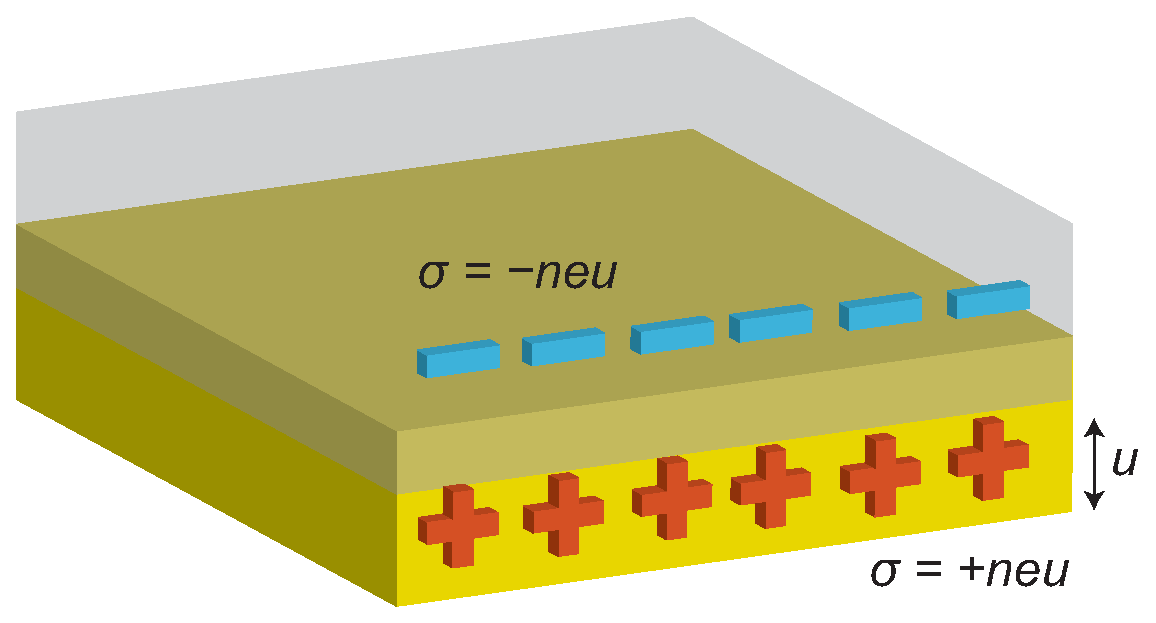
\includegraphics[scale=0.5]{THM/bulk.eps}
\caption{\label{fig:bulk}Longitudinal collective oscillations of the conduction electrons of a metal (Volume plasmons)}
\end{figure}
 We can derive plasma frequency $\omega_p$ from the simple harmonics oscillation model, a collective displacement of the electron cloud by a distance $u$ leads to a surface charge density $\sigma = \pm neu$ at the slab boundaries. This establishes a homogeneous electric field $\mathbf{E} = \frac{neu}{\varepsilon_0}$ inside the slab. Thus, the displaced electrons experience a restoring force, and their movement can be described by the equation of motion $nm\ddot{u} = -ne\mathbf{E}$. Inserting the expression for the electric field, this leads to
 \begin{subequations}
 \begin{align}
 nm\ddot{u} = -\frac{n^2e^2u}{\varepsilon_0} \\
 \ddot{u} + {\omega_p}^{2}u = 0\text{.}
 \end{align}
 \end{subequations}
  The plasma frequency $\omega_p = \sqrt{\frac{ne^2}{\varepsilon_0m}}$ can thus be recognized as the natural frequency of a free oscillation of the electron sea. The quanta of these charge oscillations are called plasmons. Due to the longitudinal nature of the excitation, volume plasmons do not couple to transverse electromagnetic waves, and can only be excited by particle impact. We can derive the dispersion relation of the generalization of volume plasmons, traveling plasma waves, from curl electric field equations (Equations~\ref{eq:curlE})
 \begin{subequations}
 \begin{align}
 \curl{\curl \mathbf{E}} &= -\mu_0 \frac{\partial^2\mathbf{D}}{\partial t^2}\label{eq:curlE}\\
\mathbf{K}( \mathbf{K}\cdot \mathbf{E}-K^{ 2 }\mathbf{E} ) &=-\varepsilon ( \mathbf{K},\omega  ) \frac { { \omega  }^{ 2 } }{ { c }^{ 2 } } \mathbf{E}
 \end{align}
 \end{subequations}  
and plasma model, and a simple equation of motion for an electron of the plasma subjected to an external electric field $\mathbf{E}$
 \begin{equation}
m\ddot{\mathbf{x}} + m\gamma\dot{\mathbf{x}} = -e\mathbf{E}\text{.}
\end{equation}
Assuming a harmonic time dependence $\mathbf{E}( t )=\mathbf{E}_0\mathrm{e}^{-i\omega t}$ of the driving field, a particular solution of this equation describing the oscillation of the electron is $\mathbf{x} ( t ) = \mathbf{x}_0 \mathrm{e}^{-i\omega t} $. The complex amplitude $\mathbf{x}_0$ incorporates any phase shifts between driving field and response via
\begin{equation}
\mathbf{x} ( t ) = \frac{e}{m( \omega^2 + i\gamma\omega )}\mathbf{E}( t )\text{.}
\end{equation}
The displaced electrons contribute to the macroscopic polarization
\begin{equation}
\mathbf{P}=-\frac{ne^2}{m( \omega^2 + i\gamma\omega )}\mathbf{E}( t )\text{.}
\end{equation}
Inserting $\mathbf{P}$ into dielectric displacement field equation $\mathbf{D} = \varepsilon_0\mathbf{E} + \mathbf{P}$ yields
\begin{equation}
\mathbf{D} = \varepsilon_0(1-\frac{\omega_p^2}{\omega^2 + i\gamma\omega})\mathbf{E}\text{,}
\end{equation}
where $\omega_p^2 = \frac{ne^2}{\varepsilon_0m}$. Therefore, the dielectric function of the free electron gas
\begin{equation}
\varepsilon(\omega) = 1- \frac{\omega_p^2}{\omega^2 + i\gamma\omega}\text{.}\label{eq:dielefu}
\end{equation}
We arrive at the desired result by using equation~\ref{eq:dielefu} and the generic dispersion relation $K^2=\varepsilon(\mathbf{K},\omega)\frac{\omega^2}{c^2}$, the dispersion relation of traveling waves becomes
\begin{equation}
\omega^2 = \omega_p^2 + \mathbf{K}^2c^2\text{.}
\end{equation}
From this relation, we can figure out the oscillation properties in any frequency of external field. Note that this branch can not confine the electromagnetic waves, it would radiate out the energy, so this mode is also called radiative surface plasmon.

\section{Surface plasmon polaritons at interface between dielectric and metal}

Surface plasmon polaritons (SPPs) are eigenmodes of transverse magnetic (TM) waves, which coupling the electromagnetic fields to oscillations of the conductor's electron plasma, propagate at a interface between dielectric and metal, and are confined in perpendicular direction. Providing a flat interface between dielectric and metal half-spaces with dielectric constants $\varepsilon_d$ and $\varepsilon_m$ , respectively, and assuming the interface normal to z direction and the SPPs propagate along the $x$ direction, the SPP wave vector $\beta$ is related to the frequency $\omega$ through the dispersion relation
\begin{equation}
\beta = k_0\sqrt{\frac{\varepsilon_d\varepsilon_m}{\varepsilon_d + \varepsilon_m}}\text{,}\label{eq:sppsdisp}
\end{equation}
where $k_0 = \omega/c$ is the free-space wave vector. We take $\omega$ to be real and allow $\beta$ to be complex.

The optical response of metals is often described by the Drude model for a free-electron gas~\cite{kittel1976introduction},
\begin{equation}
\varepsilon_{Drude}(\omega)=1-\frac{\omega_p^2}{\omega^2+i\Gamma\omega}\text{,}
\end{equation}
in which $\Gamma$ is a damping rate due to electron-electron and electron-phonon scattering.
Figure~\ref{fig:SPPdisp} shows the dispersion curve~\ref{eq:sppsdisp} with Drude metal  in the absence of losses ($\Gamma=0$) for air ($\varepsilon_d = 1$) and fused silica ($\varepsilon_d = 2.25$) interface.
\begin{figure}[htb]
\centering
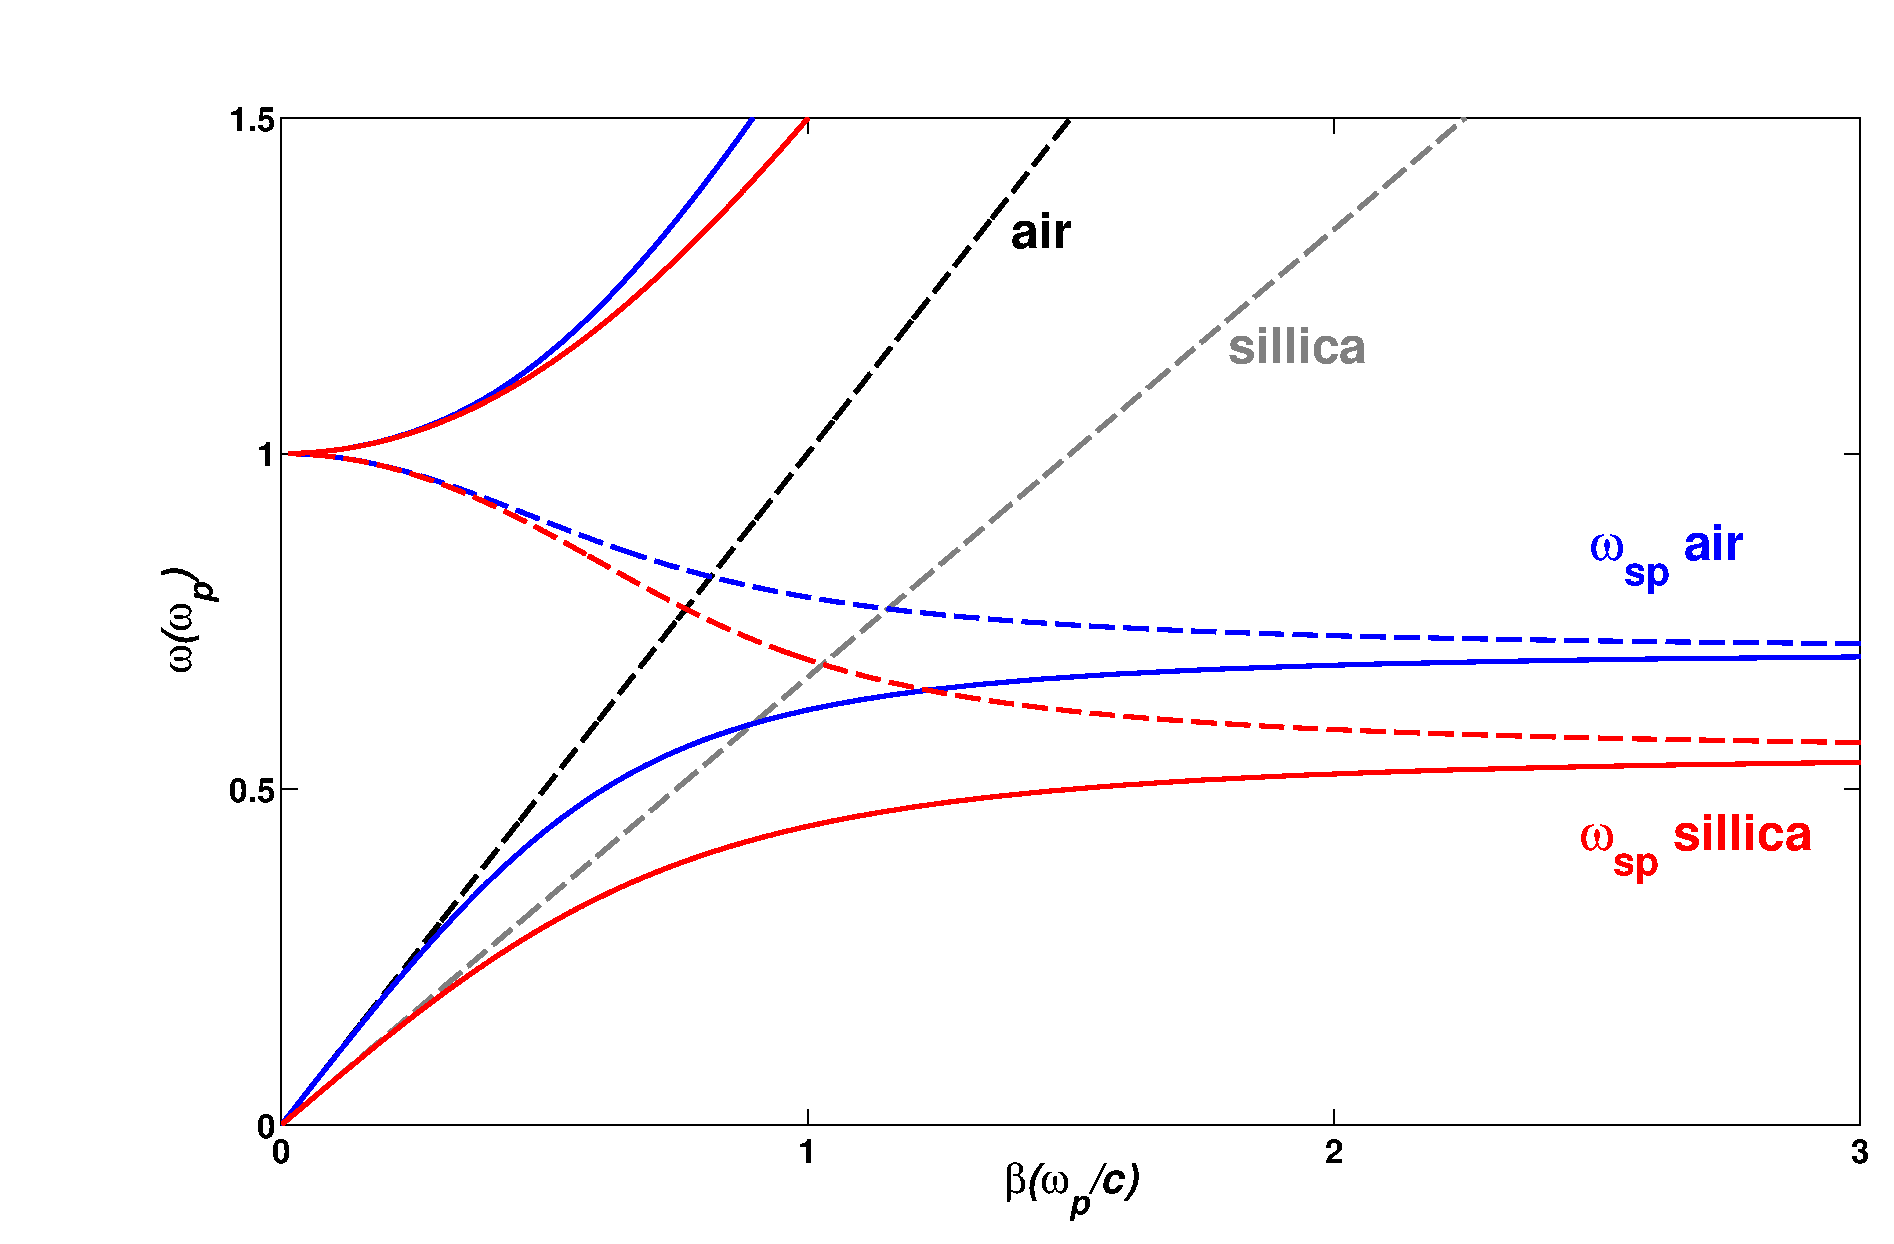
\includegraphics[scale=0.4]{THM/SPPdisp.eps}
\caption{\label{fig:SPPdisp}Dispersion relation of SPPs at the interface between a Drude metal with negligible collision frequency and air (blue curves) and silica (red curves).}
\end{figure}
For small wave vectors SPPs propagation constant $\beta$ is close to $k_0$ at the light line, in the opposite regime of the frequency close to surface plasmon frequency $\omega_p$. It also shows that the SPPs line lying to the right of the respective light lines of air and silica, so that SPPs are directed by light due to phase mismatching. The wave vector mismatch between SPPs and radiation modes needs to be overcome in order to excite or detect SPPs. This can be achieved by multiple methods~\cite{raether1988surface}. In the Otto configuration, light in a prism that is brought in close vicinity to a metal surface can excite SPPs through coupling to the evanescent field. Because light in the prism has a larger wave vector than that in air, it can be phase-matched to the SPPs. In the related Kretschmann-Raether geometry, coupling to SPPs occurs through a metal film that is deposited on a prism. In the grating coupling configuration, metal surface with a shallow grating of grooves or holes with lattice constant $a$. For the simple 1D grating of grooves depicted in Figure~\ref{fig:grating},
\begin{figure}[htb]
\centering
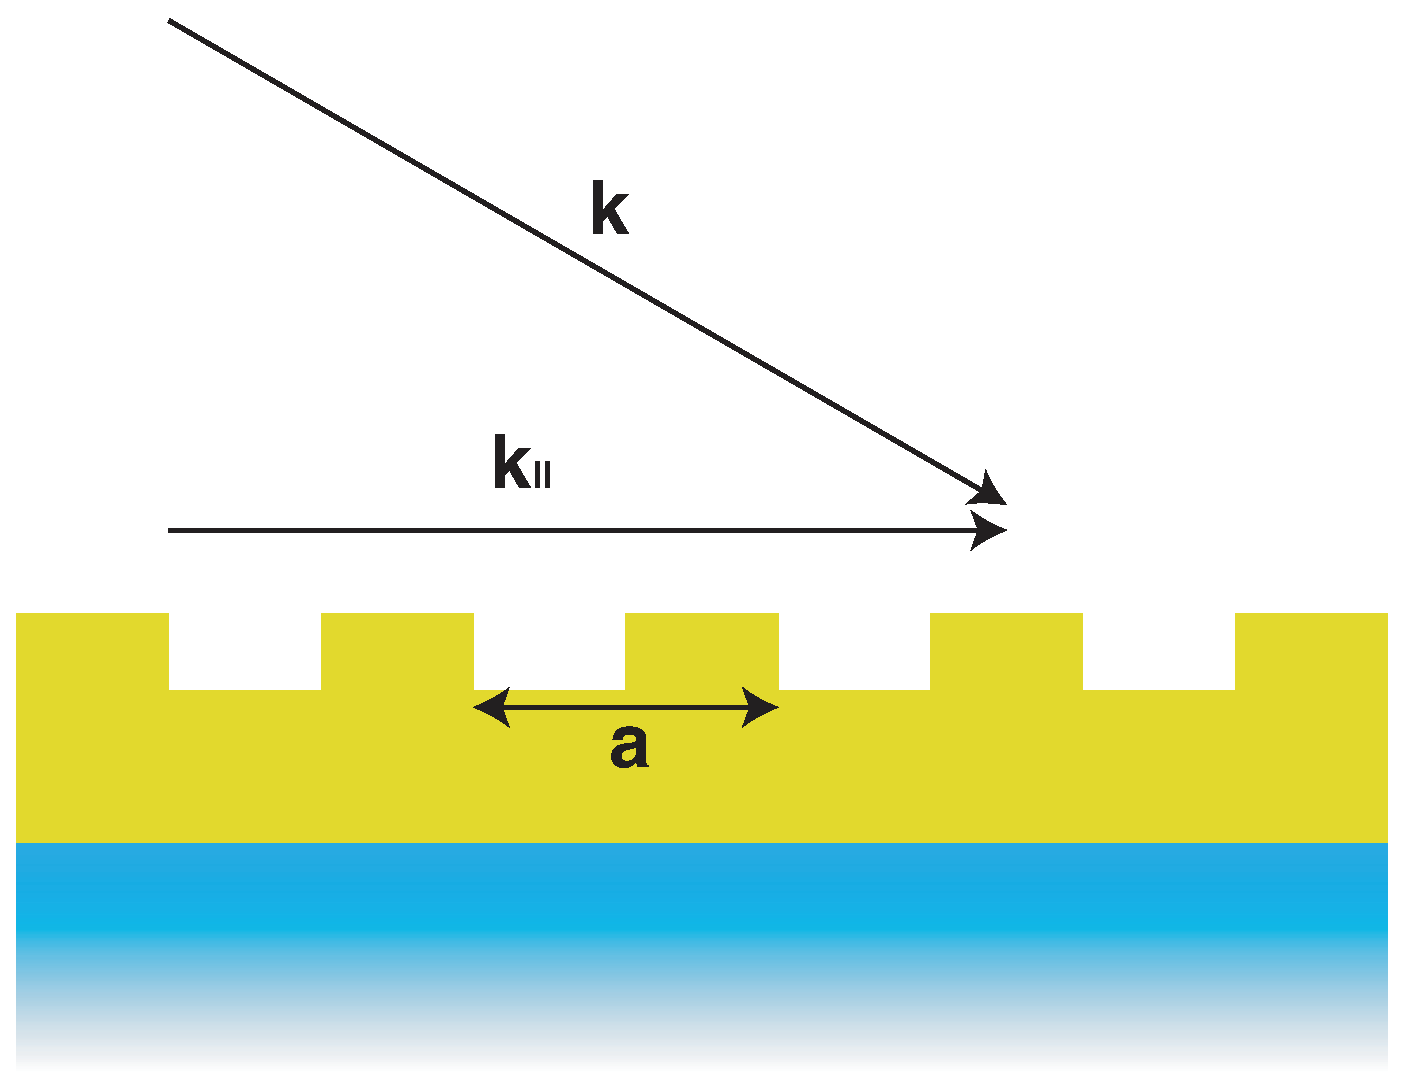
\includegraphics[scale=0.5]{THM/grating.eps}
\caption{\label{fig:grating}Phase-matching of light to SPPs the grating coupling configuration.}
\end{figure}
phase-matching takes place when the condition is fulfilled
\begin{equation}
\beta = k_0 \sin{\theta} \pm \nu g\text{,}
\end{equation}
where $g=\frac{2\pi}{a}$ is the reciprocal vector of the grating, and $\nu=(1,2,3\dots)$.
As with prism coupling, excitation of SPPs is detected as a minimum in the reflected light. The reverse process can also take place, SPPs propagating along a surface modulated with a grating can couple to light and thus radiate. 

%\bibliographystyle{unsrt}
%\bibliography{thesisbib}           =>  \chapter{Theory of surface plasmon polaritons in metallic nano-structures}
\label{c:thm}
\section{Definition of plasmon}

Plasmon is collective oscillation of conduction electron gas, a quasi-particle resulting from the quantization of plasma oscillations just like phonons are quantizations of mechanical vibrations. The simplest case is the volume plasmon as shown in Figure~\ref{fig:bulk}.
\begin{figure}[htb]
\centering
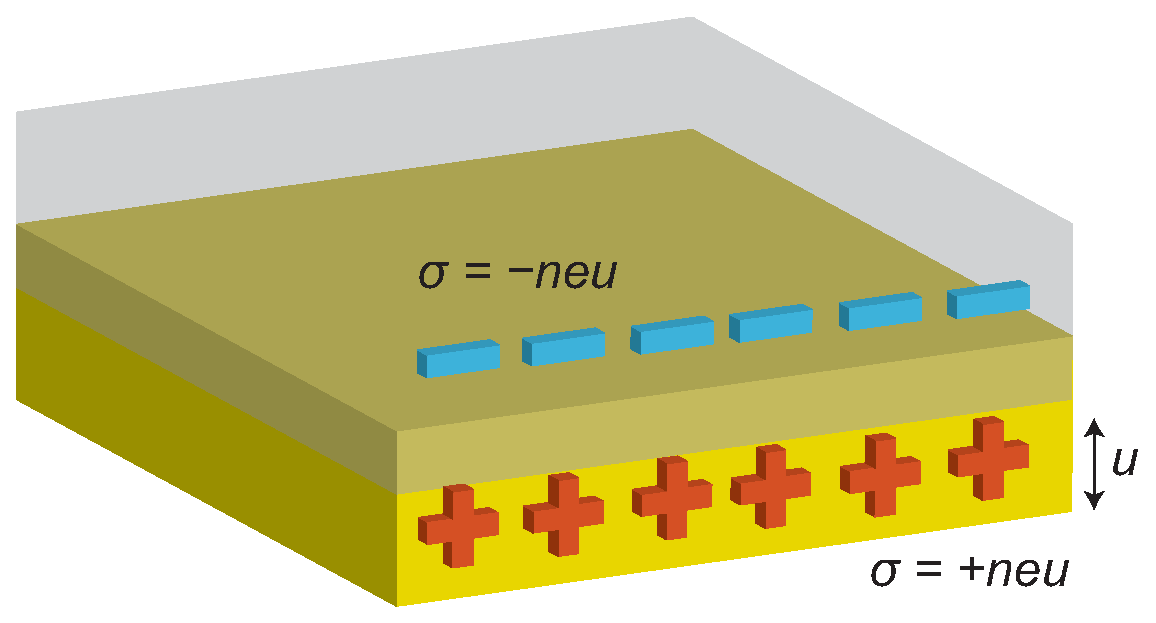
\includegraphics[scale=0.5]{THM/bulk.eps}
\caption{\label{fig:bulk}Longitudinal collective oscillations of the conduction electrons of a metal (Volume plasmons)}
\end{figure}
 We can derive plasma frequency $\omega_p$ from the simple harmonics oscillation model, a collective displacement of the electron cloud by a distance $u$ leads to a surface charge density $\sigma = \pm neu$ at the slab boundaries. This establishes a homogeneous electric field $\mathbf{E} = \frac{neu}{\varepsilon_0}$ inside the slab. Thus, the displaced electrons experience a restoring force, and their movement can be described by the equation of motion $nm\ddot{u} = -ne\mathbf{E}$. Inserting the expression for the electric field, this leads to
 \begin{subequations}
 \begin{align}
 nm\ddot{u} = -\frac{n^2e^2u}{\varepsilon_0} \\
 \ddot{u} + {\omega_p}^{2}u = 0\text{.}
 \end{align}
 \end{subequations}
  The plasma frequency $\omega_p = \sqrt{\frac{ne^2}{\varepsilon_0m}}$ can thus be recognized as the natural frequency of a free oscillation of the electron sea. The quanta of these charge oscillations are called plasmons. Due to the longitudinal nature of the excitation, volume plasmons do not couple to transverse electromagnetic waves, and can only be excited by particle impact. We can derive the dispersion relation of the generalization of volume plasmons, traveling plasma waves, from curl electric field equations (Equations~\ref{eq:curlE})
 \begin{subequations}
 \begin{align}
 \curl{\curl \mathbf{E}} &= -\mu_0 \frac{\partial^2\mathbf{D}}{\partial t^2}\label{eq:curlE}\\
\mathbf{K}( \mathbf{K}\cdot \mathbf{E}-K^{ 2 }\mathbf{E} ) &=-\varepsilon ( \mathbf{K},\omega  ) \frac { { \omega  }^{ 2 } }{ { c }^{ 2 } } \mathbf{E}
 \end{align}
 \end{subequations}  
and plasma model, and a simple equation of motion for an electron of the plasma subjected to an external electric field $\mathbf{E}$
 \begin{equation}
m\ddot{\mathbf{x}} + m\gamma\dot{\mathbf{x}} = -e\mathbf{E}\text{.}
\end{equation}
Assuming a harmonic time dependence $\mathbf{E}( t )=\mathbf{E}_0\mathrm{e}^{-i\omega t}$ of the driving field, a particular solution of this equation describing the oscillation of the electron is $\mathbf{x} ( t ) = \mathbf{x}_0 \mathrm{e}^{-i\omega t} $. The complex amplitude $\mathbf{x}_0$ incorporates any phase shifts between driving field and response via
\begin{equation}
\mathbf{x} ( t ) = \frac{e}{m( \omega^2 + i\gamma\omega )}\mathbf{E}( t )\text{.}
\end{equation}
The displaced electrons contribute to the macroscopic polarization
\begin{equation}
\mathbf{P}=-\frac{ne^2}{m( \omega^2 + i\gamma\omega )}\mathbf{E}( t )\text{.}
\end{equation}
Inserting $\mathbf{P}$ into dielectric displacement field equation $\mathbf{D} = \varepsilon_0\mathbf{E} + \mathbf{P}$ yields
\begin{equation}
\mathbf{D} = \varepsilon_0(1-\frac{\omega_p^2}{\omega^2 + i\gamma\omega})\mathbf{E}\text{,}
\end{equation}
where $\omega_p^2 = \frac{ne^2}{\varepsilon_0m}$. Therefore, the dielectric function of the free electron gas
\begin{equation}
\varepsilon(\omega) = 1- \frac{\omega_p^2}{\omega^2 + i\gamma\omega}\text{.}\label{eq:dielefu}
\end{equation}
We arrive at the desired result by using equation~\ref{eq:dielefu} and the generic dispersion relation $K^2=\varepsilon(\mathbf{K},\omega)\frac{\omega^2}{c^2}$, the dispersion relation of traveling waves becomes
\begin{equation}
\omega^2 = \omega_p^2 + \mathbf{K}^2c^2\text{.}
\end{equation}
From this relation, we can figure out the oscillation properties in any frequency of external field. Note that this branch can not confine the electromagnetic waves, it would radiate out the energy, so this mode is also called radiative surface plasmon.

\section{Surface plasmon polaritons at interface between dielectric and metal}

Surface plasmon polaritons (SPPs) are eigenmodes of transverse magnetic (TM) waves, which coupling the electromagnetic fields to oscillations of the conductor's electron plasma, propagate at a interface between dielectric and metal, and are confined in perpendicular direction. Providing a flat interface between dielectric and metal half-spaces with dielectric constants $\varepsilon_d$ and $\varepsilon_m$ , respectively, and assuming the interface normal to z direction and the SPPs propagate along the $x$ direction, the SPP wave vector $\beta$ is related to the frequency $\omega$ through the dispersion relation
\begin{equation}
\beta = k_0\sqrt{\frac{\varepsilon_d\varepsilon_m}{\varepsilon_d + \varepsilon_m}}\text{,}\label{eq:sppsdisp}
\end{equation}
where $k_0 = \omega/c$ is the free-space wave vector. We take $\omega$ to be real and allow $\beta$ to be complex.

The optical response of metals is often described by the Drude model for a free-electron gas~\cite{kittel1976introduction},
\begin{equation}
\varepsilon_{Drude}(\omega)=1-\frac{\omega_p^2}{\omega^2+i\Gamma\omega}\text{,}
\end{equation}
in which $\Gamma$ is a damping rate due to electron-electron and electron-phonon scattering.
Figure~\ref{fig:SPPdisp} shows the dispersion curve~\ref{eq:sppsdisp} with Drude metal  in the absence of losses ($\Gamma=0$) for air ($\varepsilon_d = 1$) and fused silica ($\varepsilon_d = 2.25$) interface.
\begin{figure}[htb]
\centering
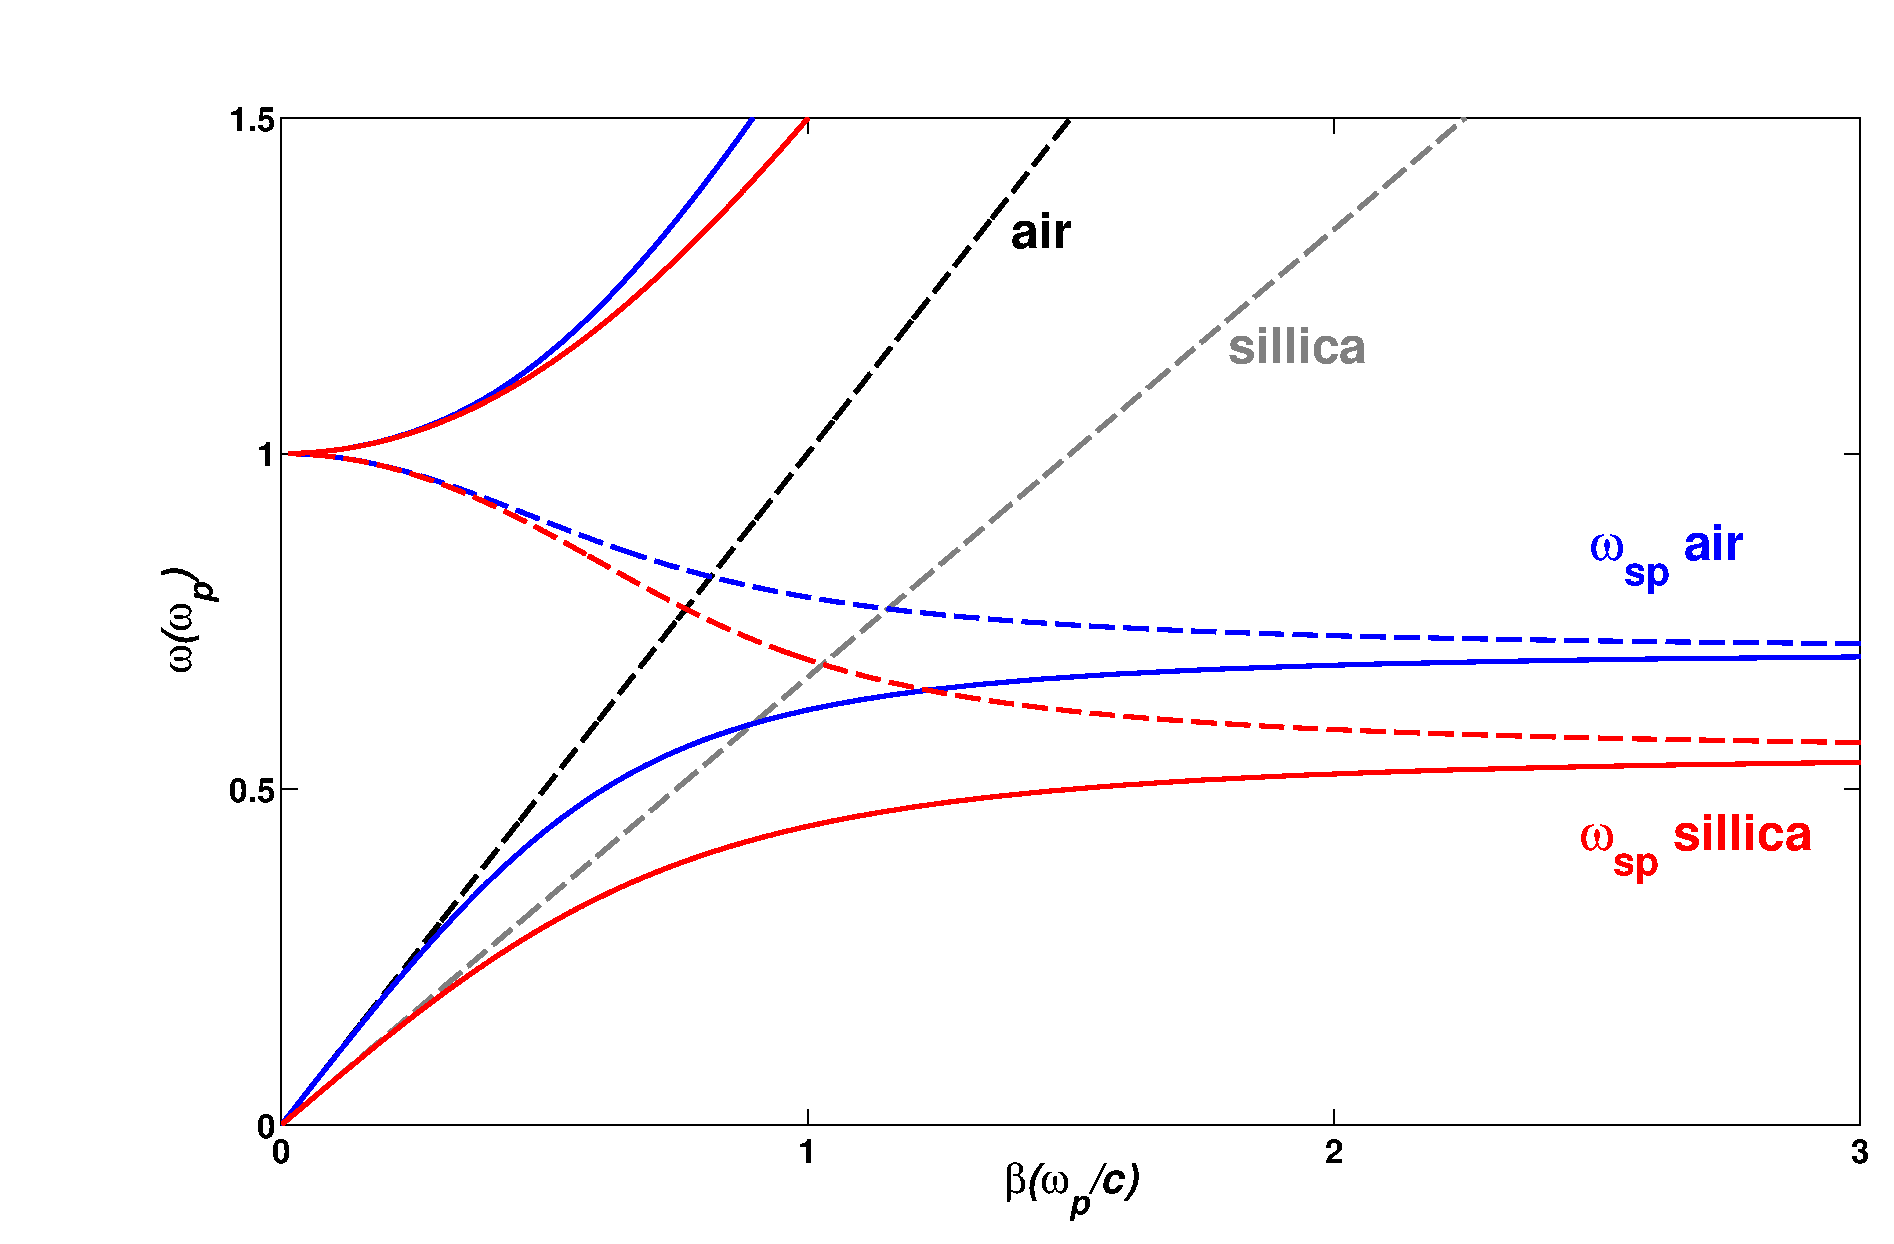
\includegraphics[scale=0.4]{THM/SPPdisp.eps}
\caption{\label{fig:SPPdisp}Dispersion relation of SPPs at the interface between a Drude metal with negligible collision frequency and air (blue curves) and silica (red curves).}
\end{figure}
For small wave vectors SPPs propagation constant $\beta$ is close to $k_0$ at the light line, in the opposite regime of the frequency close to surface plasmon frequency $\omega_p$. It also shows that the SPPs line lying to the right of the respective light lines of air and silica, so that SPPs are directed by light due to phase mismatching. The wave vector mismatch between SPPs and radiation modes needs to be overcome in order to excite or detect SPPs. This can be achieved by multiple methods~\cite{raether1988surface}. In the Otto configuration, light in a prism that is brought in close vicinity to a metal surface can excite SPPs through coupling to the evanescent field. Because light in the prism has a larger wave vector than that in air, it can be phase-matched to the SPPs. In the related Kretschmann-Raether geometry, coupling to SPPs occurs through a metal film that is deposited on a prism. In the grating coupling configuration, metal surface with a shallow grating of grooves or holes with lattice constant $a$. For the simple 1D grating of grooves depicted in Figure~\ref{fig:grating},
\begin{figure}[htb]
\centering
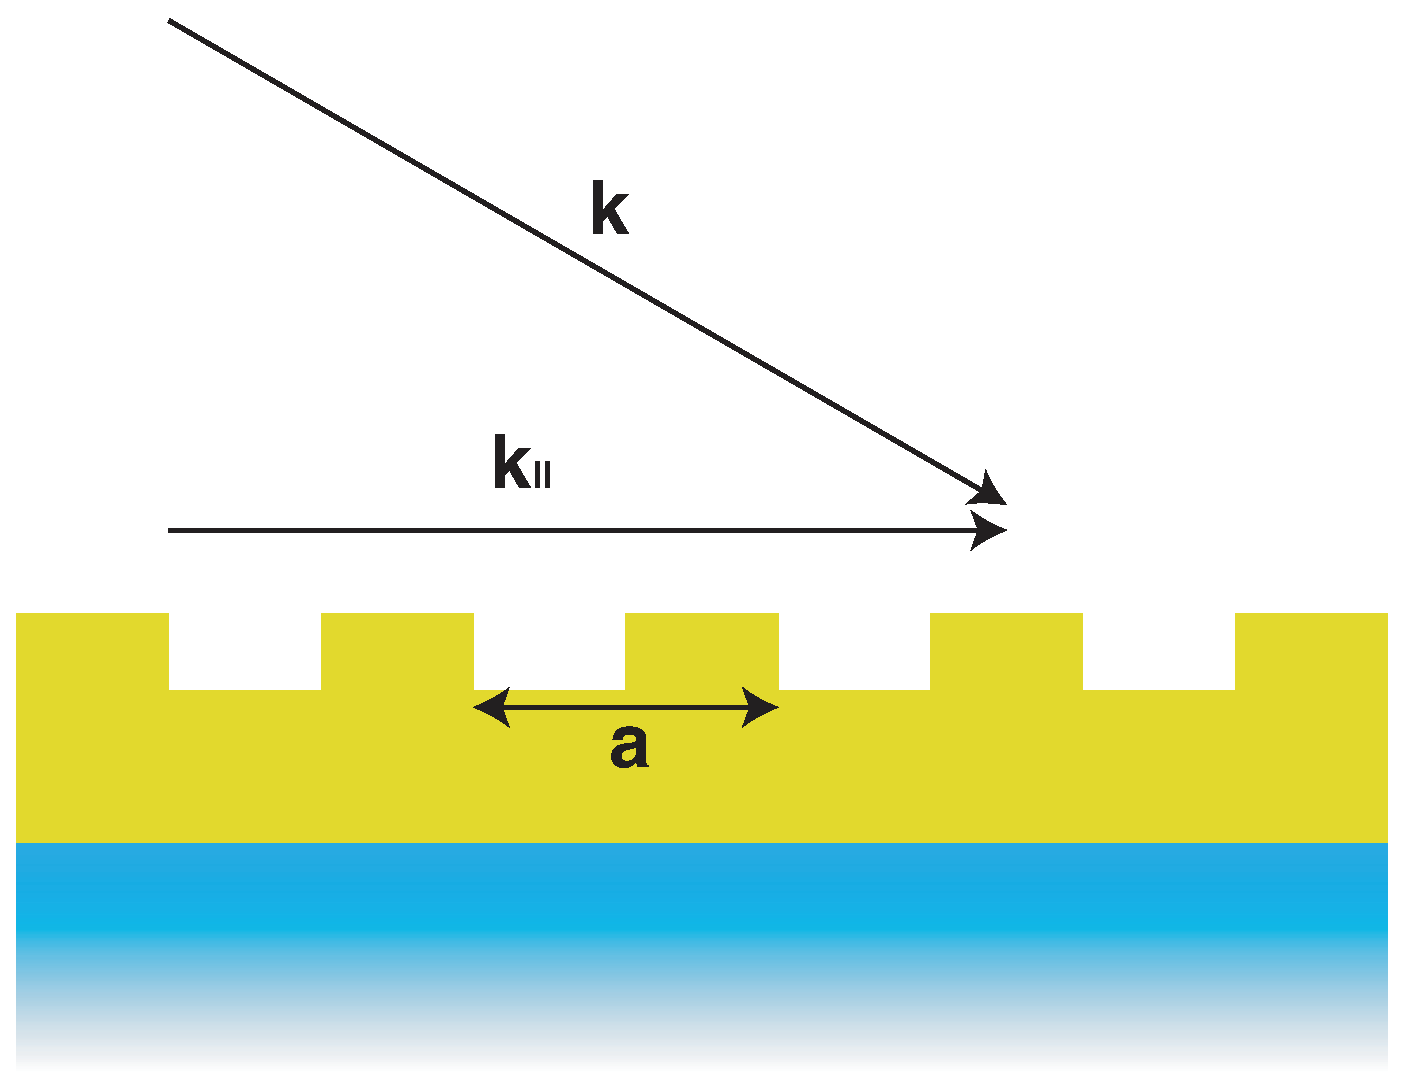
\includegraphics[scale=0.5]{THM/grating.eps}
\caption{\label{fig:grating}Phase-matching of light to SPPs the grating coupling configuration.}
\end{figure}
phase-matching takes place when the condition is fulfilled
\begin{equation}
\beta = k_0 \sin{\theta} \pm \nu g\text{,}
\end{equation}
where $g=\frac{2\pi}{a}$ is the reciprocal vector of the grating, and $\nu=(1,2,3\dots)$.
As with prism coupling, excitation of SPPs is detected as a minimum in the reflected light. The reverse process can also take place, SPPs propagating along a surface modulated with a grating can couple to light and thus radiate. 

%\bibliographystyle{unsrt}
%\bibliography{thesisbib}
\chapter{Experiment}
\label{c:exp}

\section{Atomic force microscopy}

\begin{figure}[htb]
\centering
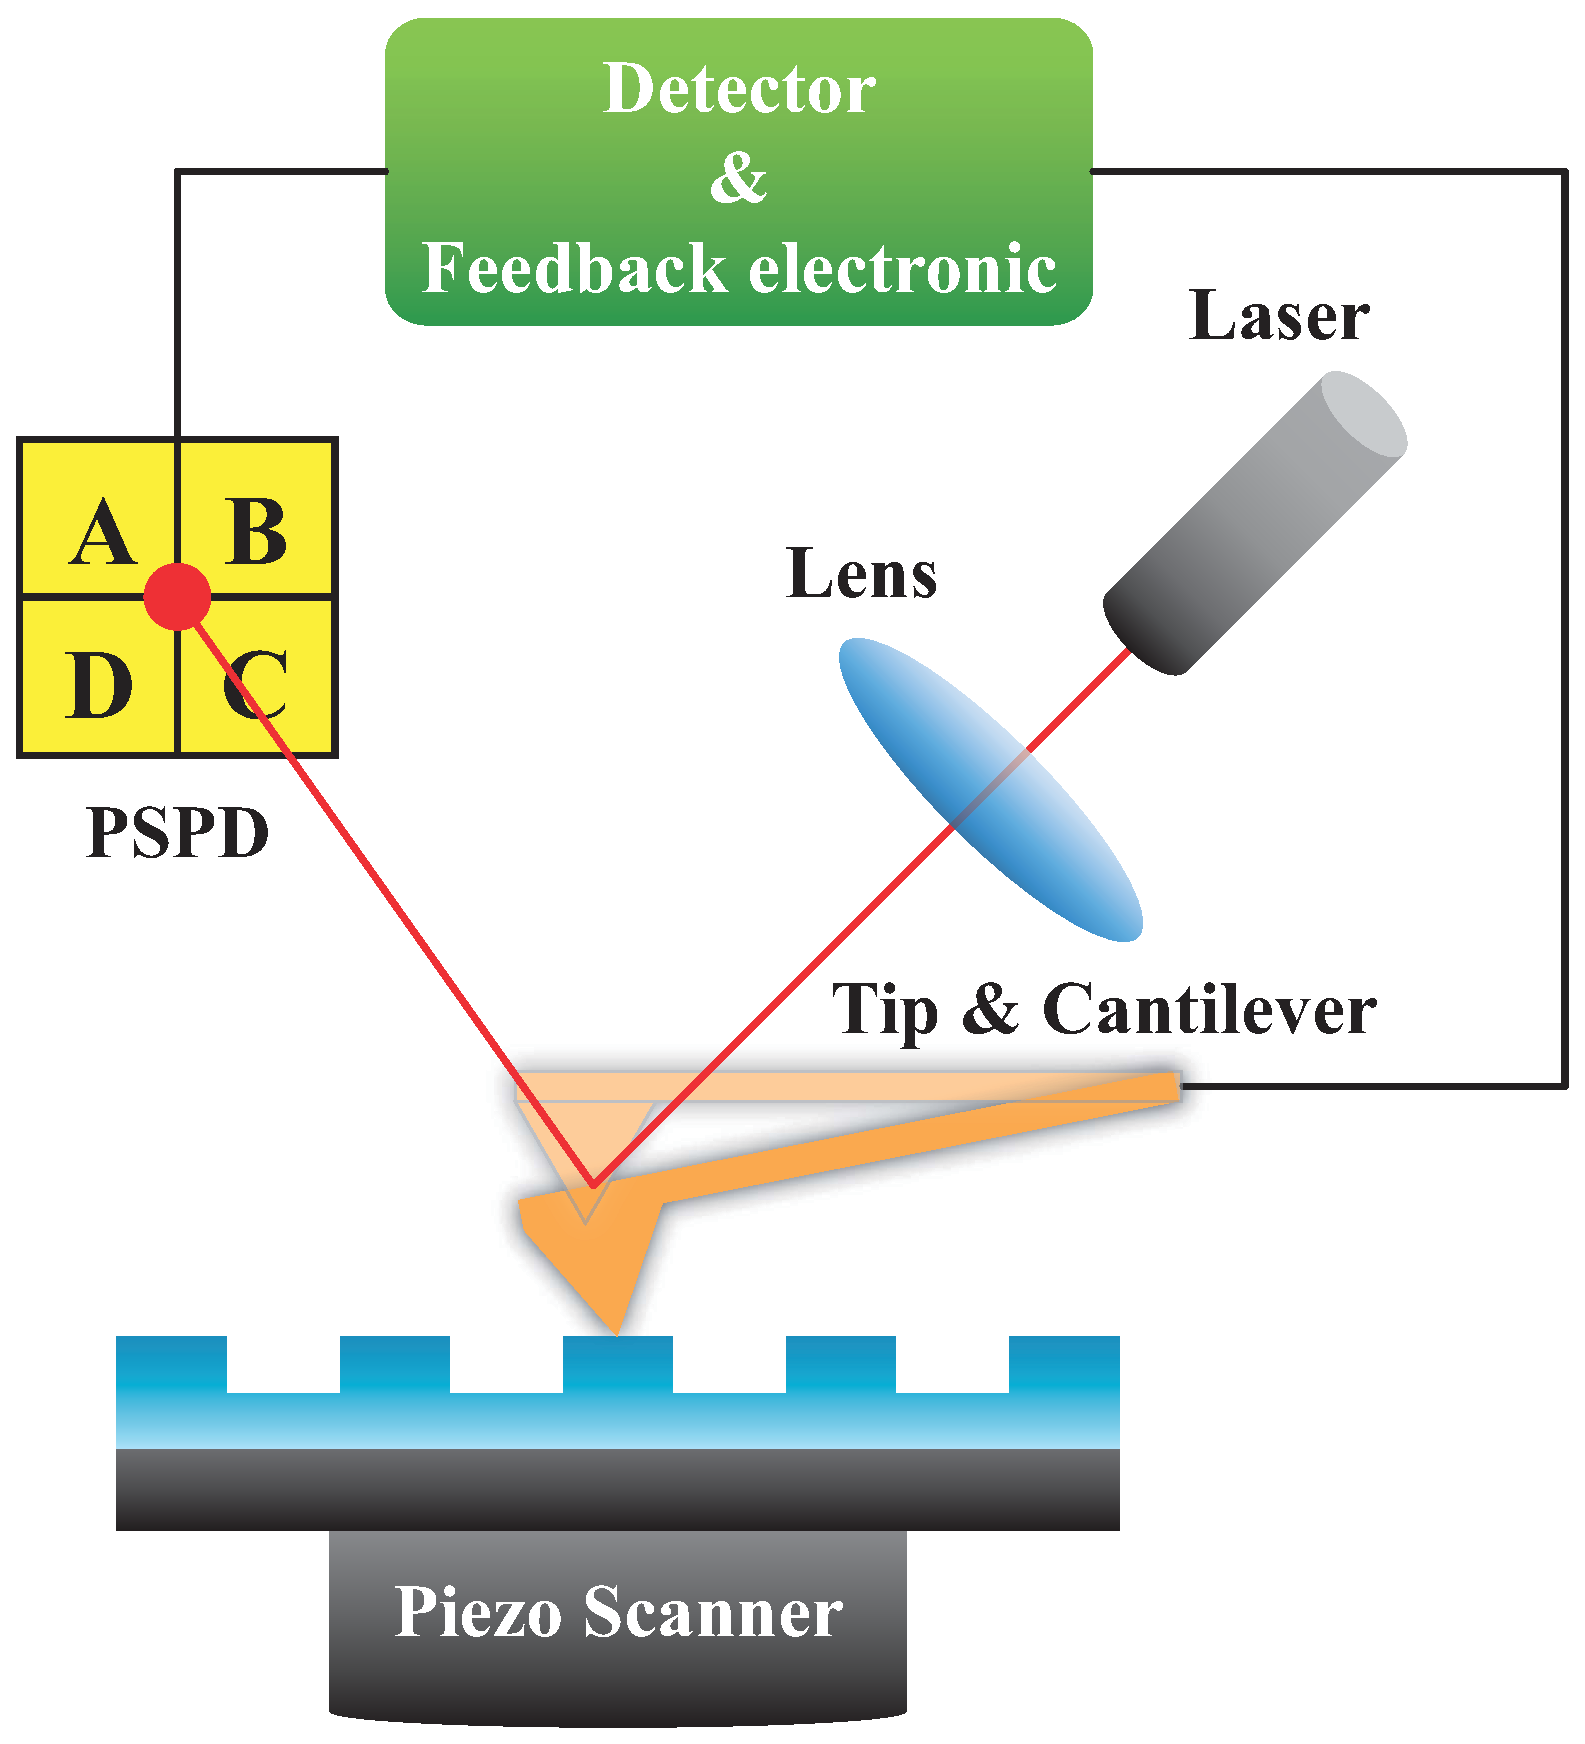
\includegraphics[scale=0.35]{EXP/afm1.eps}
\caption{\label{fig:afm1}Schematic of atomic force microscopy.}
\end{figure}
Atomic force microscope (AFM) is a type of scanning probe microscopes (SPM)~\cite{bennig1988atomic}.  The schematic of AFM is shown in Figure~\ref{fig:afm1}. AFM operates by measuring force between a probe and the specimen surfaces. In general,  the probe is a sharp tip at a cantilever's end. The cantilever can be deflected by atomic forces to sufficiently large amount, then AFM can measure the vertical and lateral deflections of the cantilever by using the optical system. A laser beam is transmitted to cantilever, and the reflected laser beam is detected with a position-sensitive photo detector (PSPD). PSPD is four-sectional that allows measuring not only vertical but lateral bending too(Figure~\ref{fig:afm2}). The output of the PSPD is provided to a computer for processing of the data for providing a topographical image of the surface with atomic resolution, and controlling the height between probe and specimen surfaces by applying voltage on piezoelectric scanner.
\begin{figure}[htb]
\centering
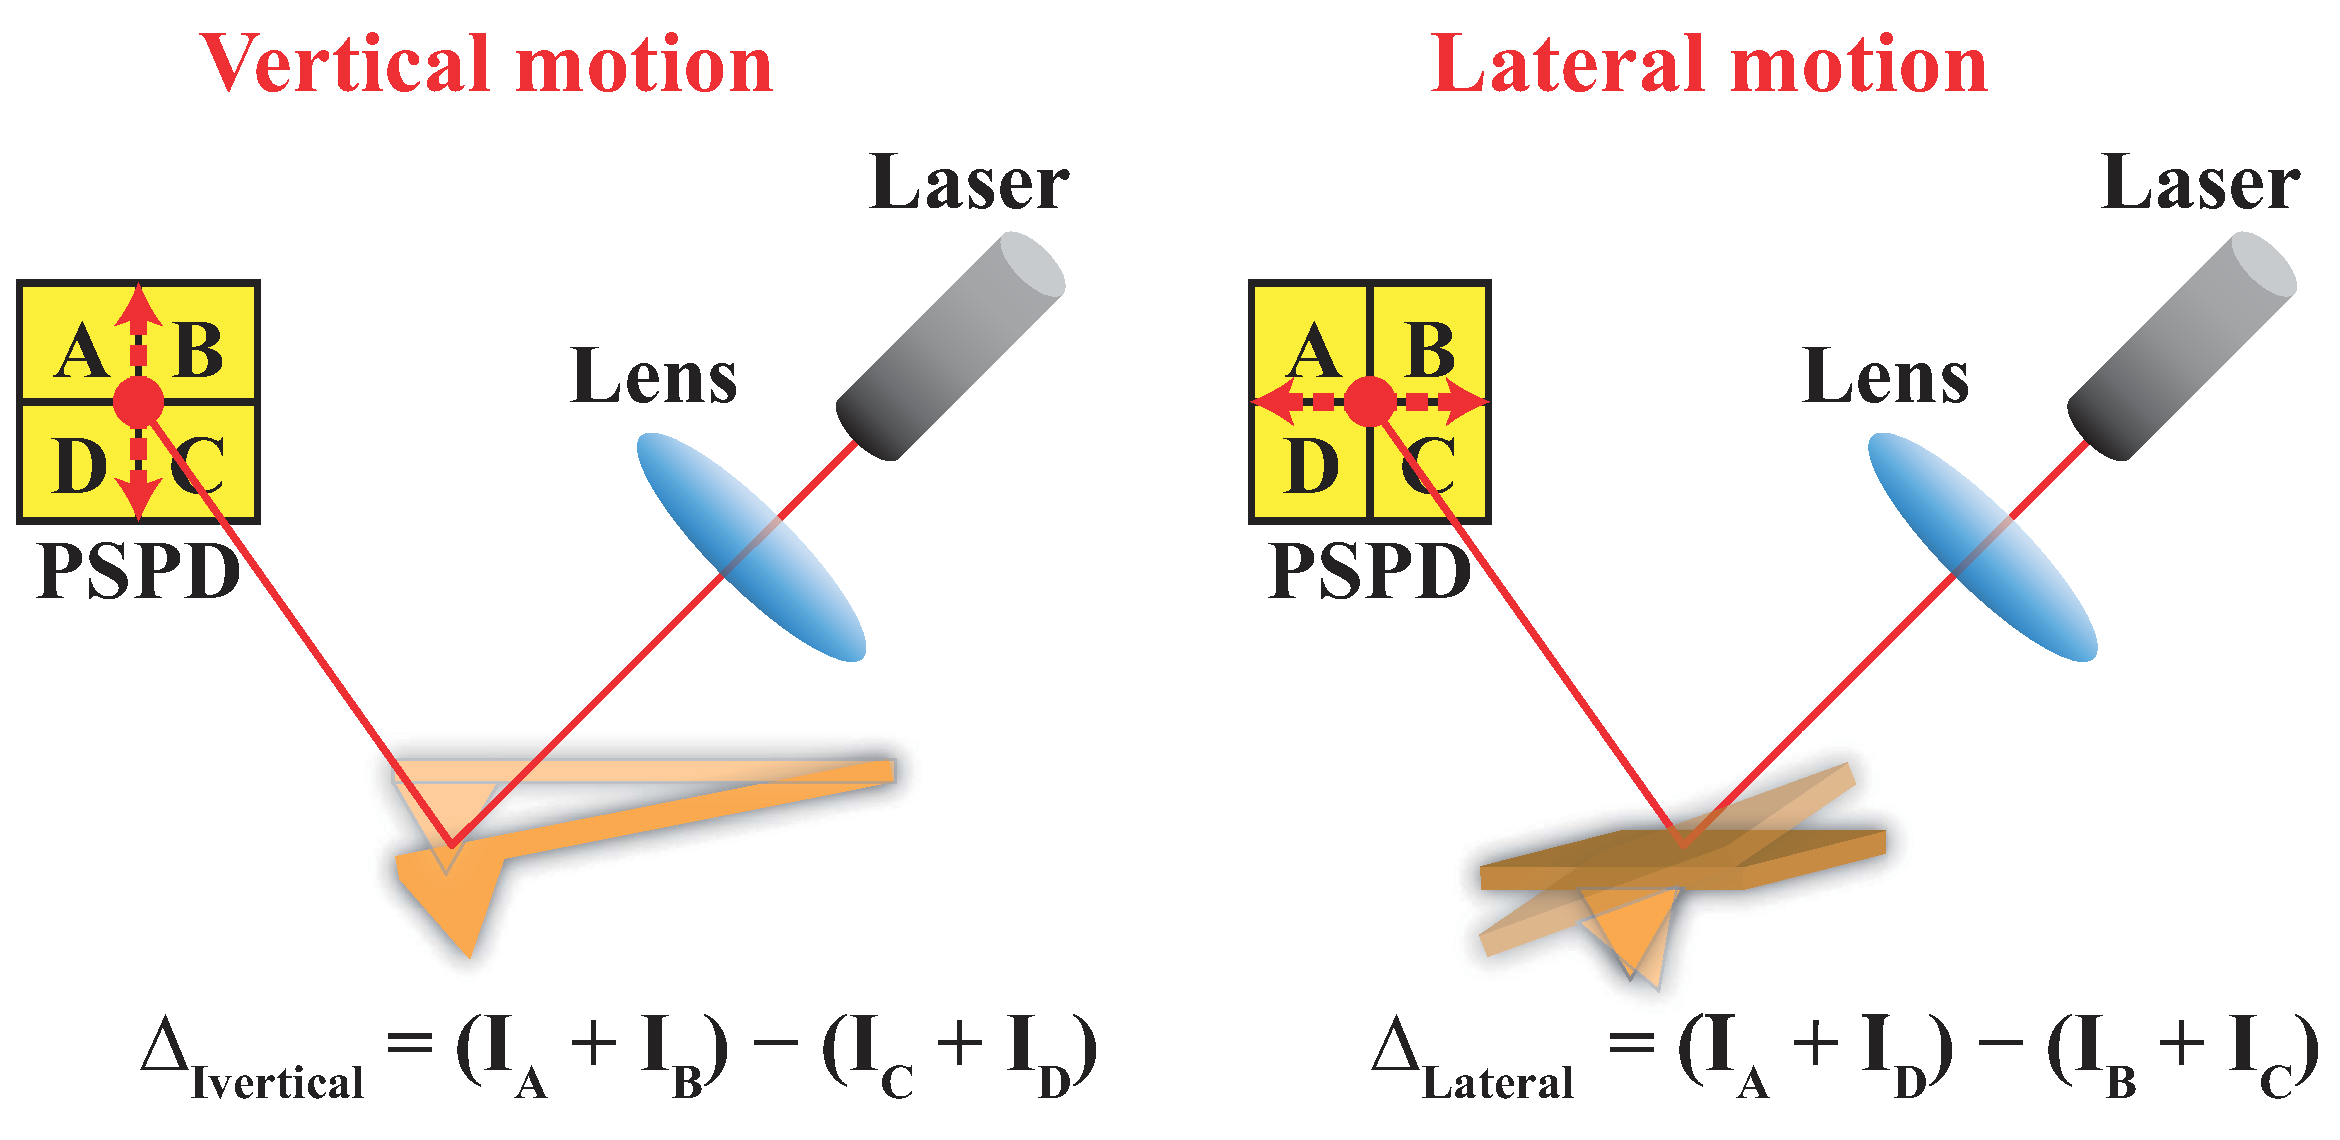
\includegraphics[scale=0.4]{EXP/afm2.eps}
\caption{\label{fig:afm2}Schematic of optical system for cantilever deflections detection.}
\end{figure}

The physical principle of the AFM operation is based on interaction between the probe tip and the specimen surface(Figure~\ref{fig:afm3}). When the cantilever approaches the specimen surface, Van der Waals forces start acting upon it . They are sufficiently far-ranging and are felt at the distance of a few tens of angstroms. Then at the distance of several angstroms repulsive force starts acting. In humid air a water layer is present on the specimen surface. The capillary force arises that holds the tip in contact with the surface and increases the minimum achievable interaction force. Electrostatic interaction between the probe and the sample may appear rather often. This can be both attraction and repulsion. Van der Waals attraction forces, capillary, electrostatic and repulsion forces at the point where the tip touches the sample and forces acting upon the tip from the deformed cantilever compensate each other in equilibrium. Based on the type and degree of this interaction the AFM modes can be broken down into contact and semi-contact(Figure~\ref{fig:afm3} ), which is a transition mode between the contact and non-contact modes.
\begin{figure}[htb]
\centering
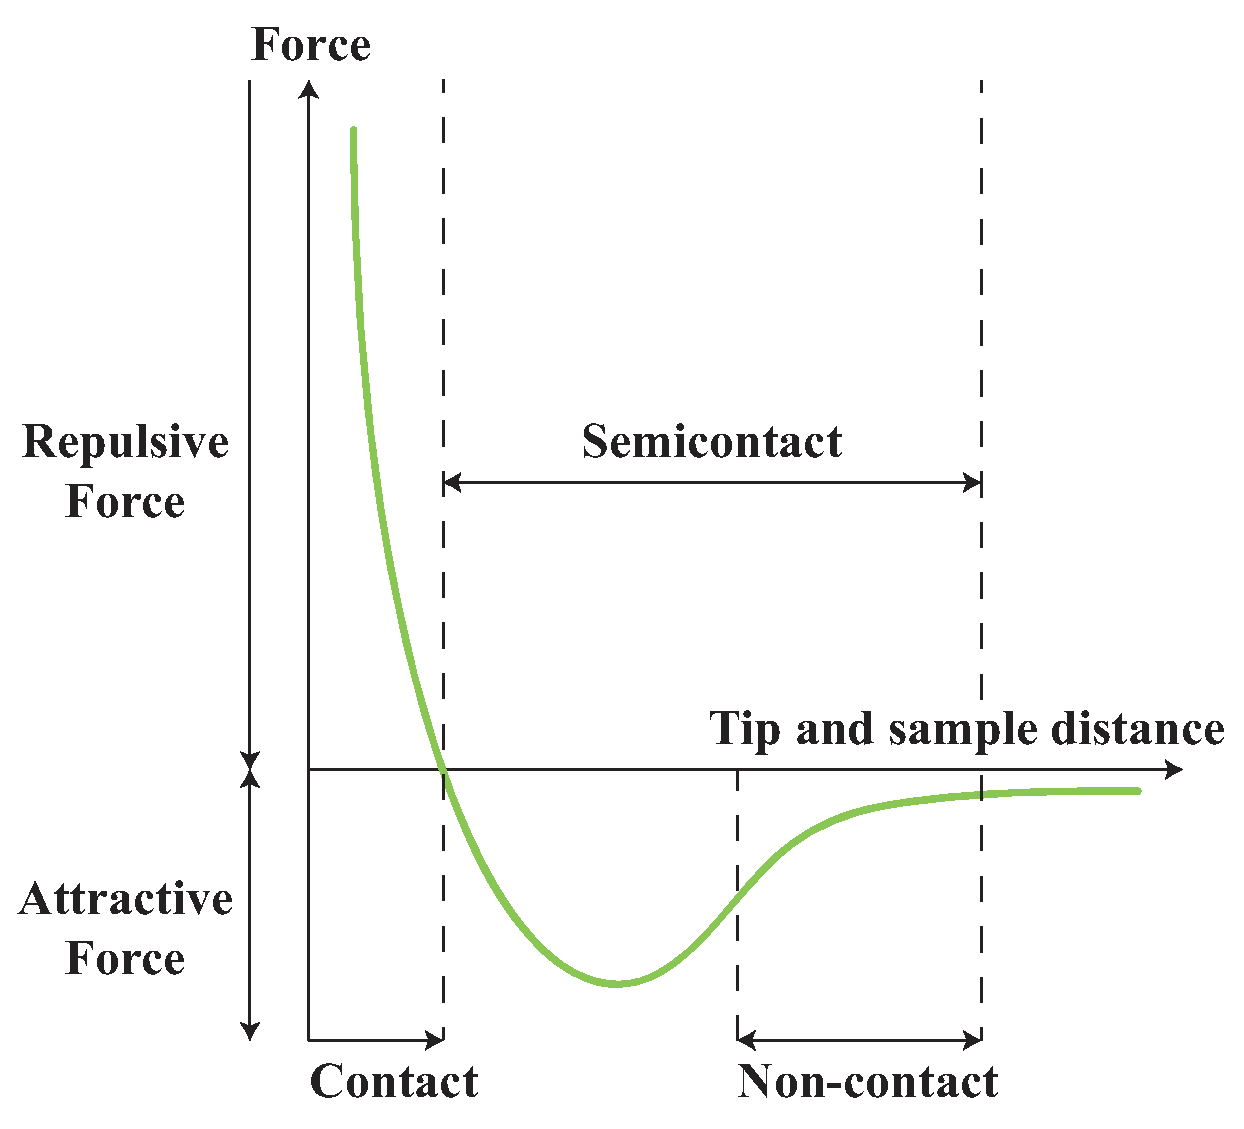
\includegraphics[scale=0.6]{EXP/afm3.eps}
\caption{\label{fig:afm3}Sketch of tip-sample forces.}
\end{figure}

\paragraph{Contact mode}

In contact mode of operation the cantilever deflection under scanning reflects repulsive force acting upon the tip. Repulsion force $\mathbf{F}$ acting upon the tip is related to the cantilever deflection value $\mathbf{x}$ under Hooke's law: $\mathbf{F}=-K \cdot  \mathbf{x}$, where $K$ is cantilever spring constant. The spring constant values for different cantilevers usually vary from 0.01 to several $\mathbf{N/m}$.

In our units the vertical cantilever deflection value is measured by means of the optical registration system and converted into electrical signal DFL (difference signal between the upper and lower halves of the PSPD) . In contact mode the DFL signal is used as a parameter characterizing the interaction force between the tip and the surface. There is a linear relationship between the DFL value and the force. In constant force mode of operation the deflection of the cantilever is maintained by the feedback circuitry on the preset value. So vertical displacement of the scanner under scanning reflects topography of sample under investigation.

Contact force microscopy is surface topography measurement in the contact mode.The microscope operation in the mode of maintaining constant interaction force between the tip and the surface sample, and is the base for measuring surface topography as well as for measuring local rigidity, local viscosity and local friction force. Constant force mode has some advantages and disadvantages. Main advantage of constant force mode is possible to measure with high resolution simultaneously with topography and some other characteristics, such as friction forces, spreading resistance etc. Constant force mode has also some disadvantages. Speed of scanning is restricted by the response time of feedback system. When exploring soft samples they can be destroyed by the scratching because the probe scanning tip is in direct contact with the surface. Therefore, under scanning soft unhomogeneous samples the local flexure of sample surface varies. As a result acquired topography of the sample can be proved distorted. Possible existence of substantial capillary forces imposed by a liquid adsorption layer can decrease the resolution.

\paragraph{Semi-contact mode}

The semi-contac mode can be characterized by some advantages in comparison with contact mode. First of all, in this mode the force of pressure of the cantilever onto the surface is less, that allows to work with softer materials such as polymers and bio-organics. The semi contact mode is also more sensitive to the interaction with the surface that gives a possibility to investigate some characteristics of the surface distribution of magnetic and electric domains, elasticity and viscosity of the surface. 

Widely used semi-contact mode has some disadvantage concerned with the usage of the feedback circuit. The scanning speed in semi-contact mode is restricted by the feedback circuit reaction time. This disadvantage can be overcome by the fact that under scanning new value of cantilever oscillation amplitude (and error signal) usually is achieved faster than preset value of the cantilever oscillation amplitude can be reached by the feedback system. Time of the reaching new value of the oscillation amplitude is determined by the oscillation period and Q-quality of the cantilever.
The feedback error signal, emerging when scanning in the semi-contact mode, contains some additional information about the topography. It can be utilized for achieving a more precise recovery of the relief. 

Additionally, similarly to the contact error mode, which can be considered as intermediate between the constant force mode and constant height mode, the feedback gain factor (i.e. the feedback processing speed) can be adjusted for the system to be able to trace subtle changes of the relief and to be too slow to trace the steep changes. Then, when the probe travels over minor irregularities, scanning will be carried out with an almost constant piezo scanner length. As a result, the slow changes of the relief will hardly show up on the images, and the steep changes will appear in high contrast. This may be helpful in finding minor irregularities on large areas against major sloping relief features. It must be noted that height of the minor irregularities must be less than amplitude of cantilever oscillation.

\section{Scanning electron microscopy}

The scanning electron microscope (SEM) is used for the observation of specimen surfaces~\cite{von1938elektronen}. When the specimen is irradiated with a fine electron beam, secondary electrons are emitted from the specimen surface. Topography of the surface can be observed by two-dimensional scanning of the electron probe over the surface and acquisition of an image from the detected secondary electrons. The concept schematic of commercial SEM (JEOL, JSM-6500F) is shown in Figure~\ref{fig:sem1}. The basic unit is composed of an electron optical system, a specimen stage, a secondary-electron detector, an image display unit, and an operation system. The electron optical system consists of an electron gun, a condenser lens and an objective lens to produce an electron probe, a scanning coil to scan the electron probe, and other components. The system inside of the microscope column are kept at vacuum.
\begin{figure}[htb]
\centering
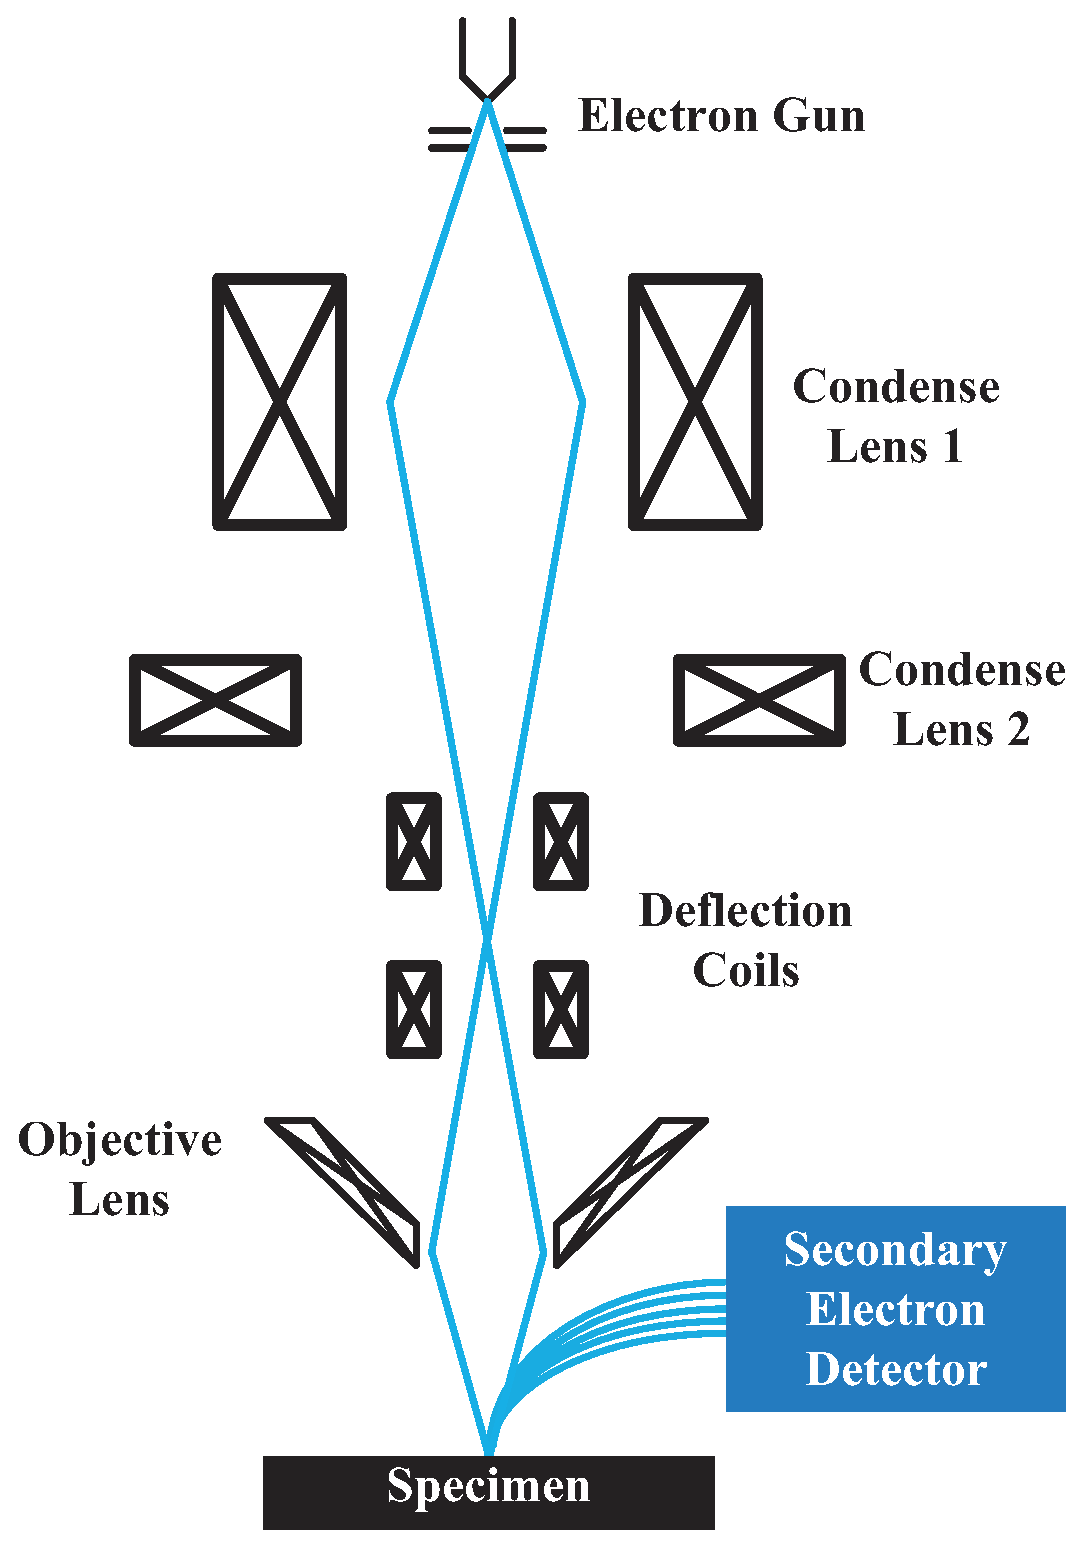
\includegraphics[scale=0.5]{EXP/SEM.eps}
\caption{\label{fig:sem1}Basic construction of a scanning electron microscopy.}
\end{figure}


The JSM-6500F utilizes a Schottky type field-emission (T-FE) gun for the electron source. The T-FE gun can constantly supply the surface of the cathode with zirconium oxide by heating the surface of cathode to 1800 K. For this reason, it can easily obtain stable and high probe current (range from several pA to 100 nA) compared with the traditional thermal emission electron gun and cold field-emission gun.

The magnetic condenser and objective lens system act to control the diameter of the beam as well as to focus the beam on the specimen due to a rotationally-symmetric magnetic field is formed when we pass a direct electric current through a coilwound electric wire in the magnetic lens. A pair of deflector coils, which between the condenser and objective lens, controlled by the scan generator, which are responsible for rastering that focused beam across the specimen surface. The size of the rastering pattern is under magnification control. The beam is rastered from left to right and top to bottom. There is a one-to-one correspondence between the rastering pattern on the specimen and the rastering pattern used to produce the image on the monitor. The resolution we choose to image at will obviously affect the number of pixels per row as well as the number of rows that constitute the scanned area.

The signal is generated from the specimen, and collected by the detector and subsequently processed to generate the image. That processing takes the intensity of the signal coming from a pixel on the specimen and converts it to a grayscale value of the corresponding monitor pixel. The monitor image is a two dimensional rastered pattern of grayscale values.

With the beam focused on the specimen surface, all we need to do to change magnification is to change the size of the rastered area on the specimen. The size of the monitor raster pattern is constant. Magnification will increase if we reduce the size of the area scanned on the specimen.

%\bibliographystyle{unsrt}
%\bibliography{thesisbib}           =>  \chapter{Experiment}
\label{c:exp}

\section{Atomic force microscopy}

\begin{figure}[htb]
\centering
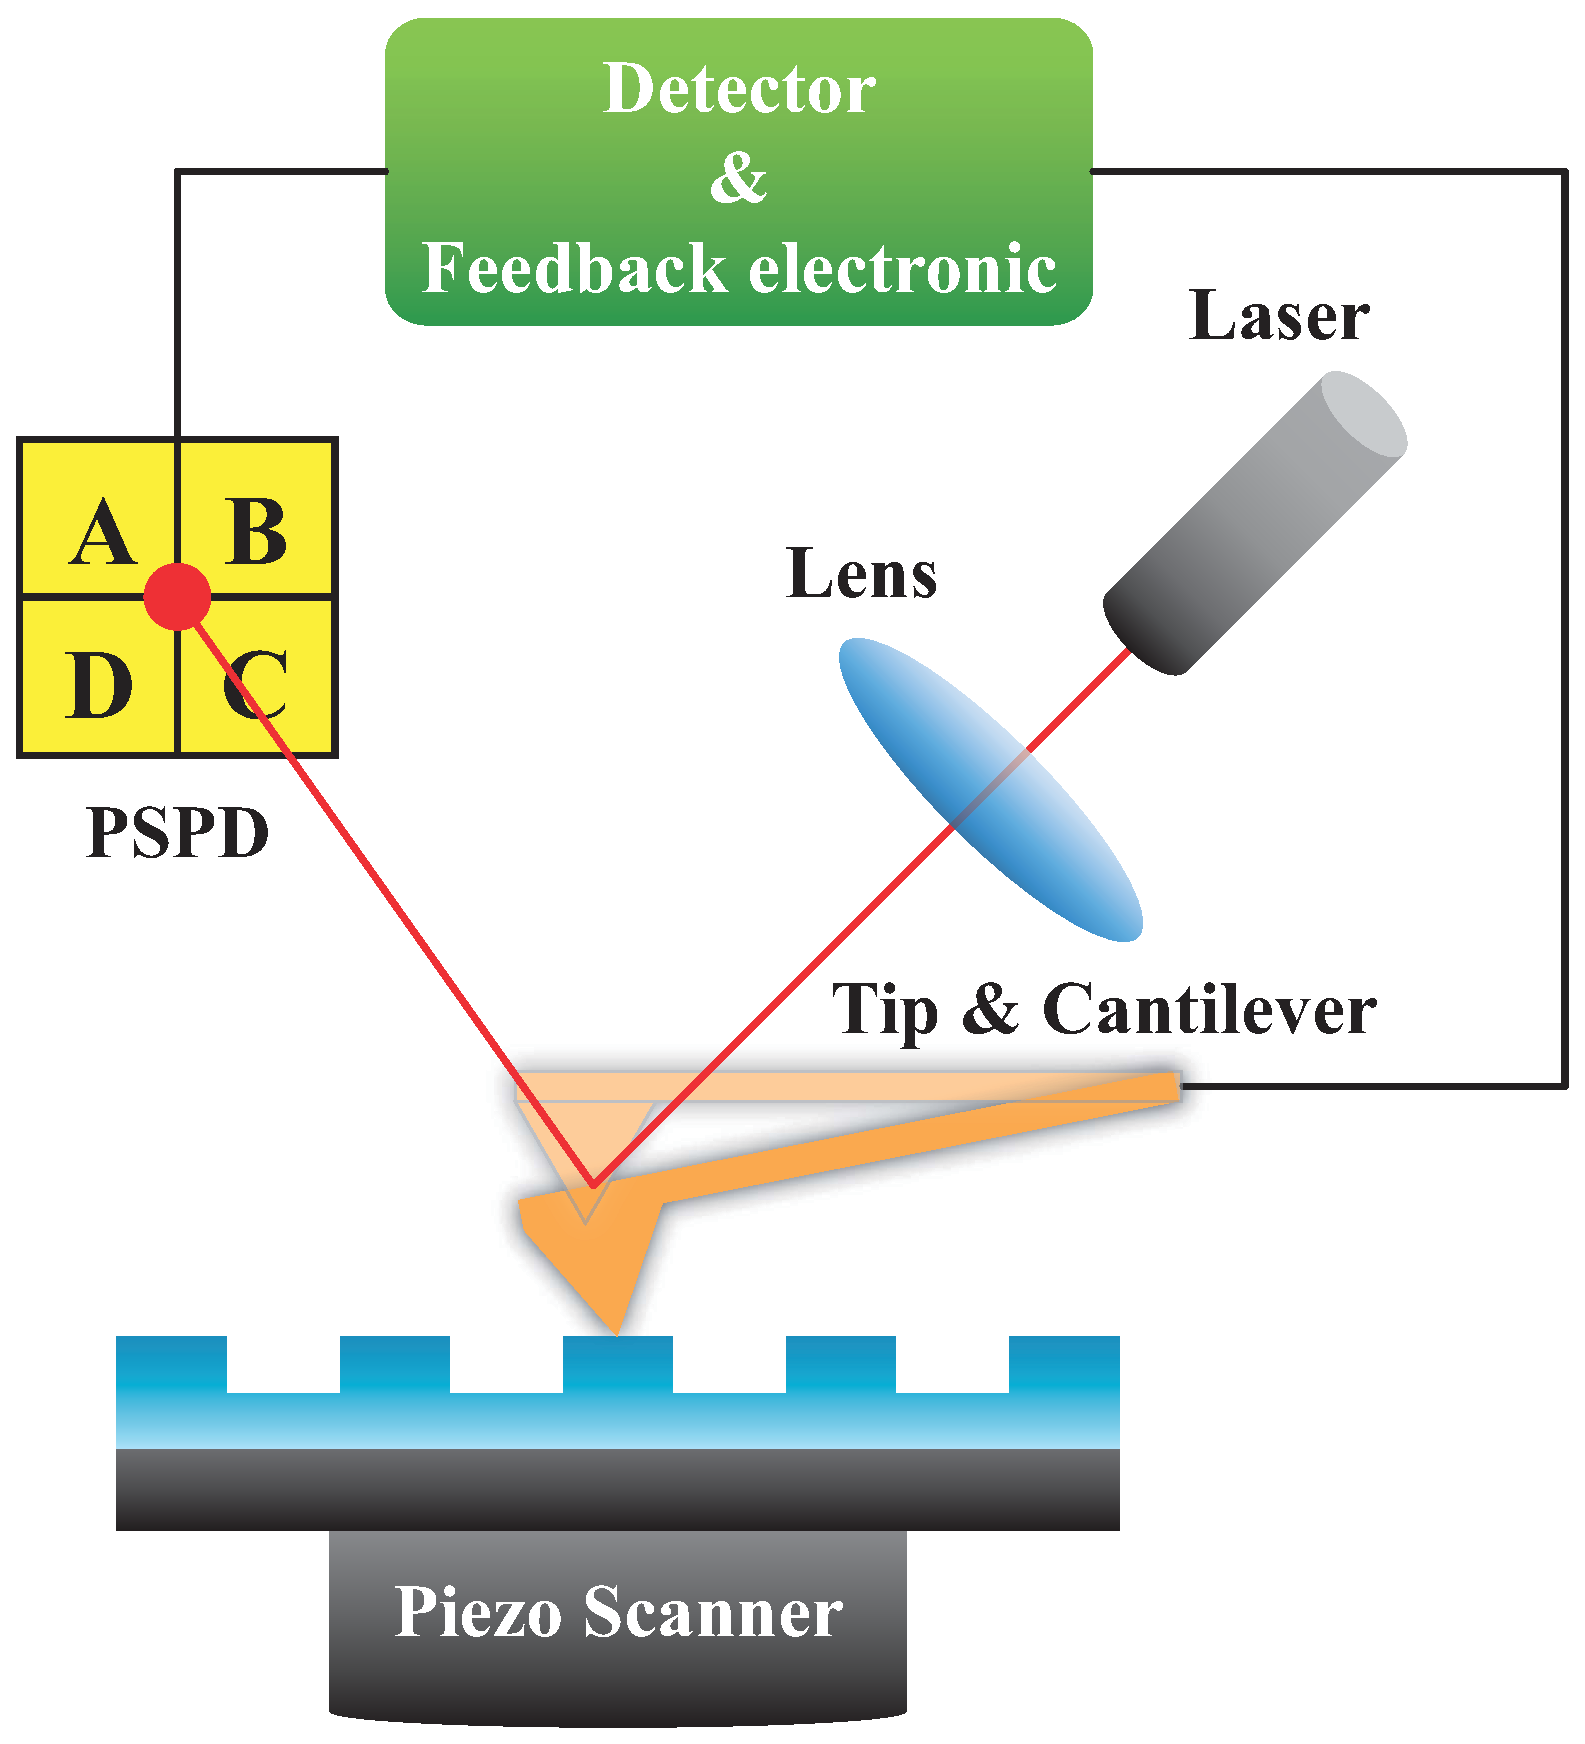
\includegraphics[scale=0.35]{EXP/afm1.eps}
\caption{\label{fig:afm1}Schematic of atomic force microscopy.}
\end{figure}
Atomic force microscope (AFM) is a type of scanning probe microscopes (SPM)~\cite{bennig1988atomic}.  The schematic of AFM is shown in Figure~\ref{fig:afm1}. AFM operates by measuring force between a probe and the specimen surfaces. In general,  the probe is a sharp tip at a cantilever's end. The cantilever can be deflected by atomic forces to sufficiently large amount, then AFM can measure the vertical and lateral deflections of the cantilever by using the optical system. A laser beam is transmitted to cantilever, and the reflected laser beam is detected with a position-sensitive photo detector (PSPD). PSPD is four-sectional that allows measuring not only vertical but lateral bending too(Figure~\ref{fig:afm2}). The output of the PSPD is provided to a computer for processing of the data for providing a topographical image of the surface with atomic resolution, and controlling the height between probe and specimen surfaces by applying voltage on piezoelectric scanner.
\begin{figure}[htb]
\centering
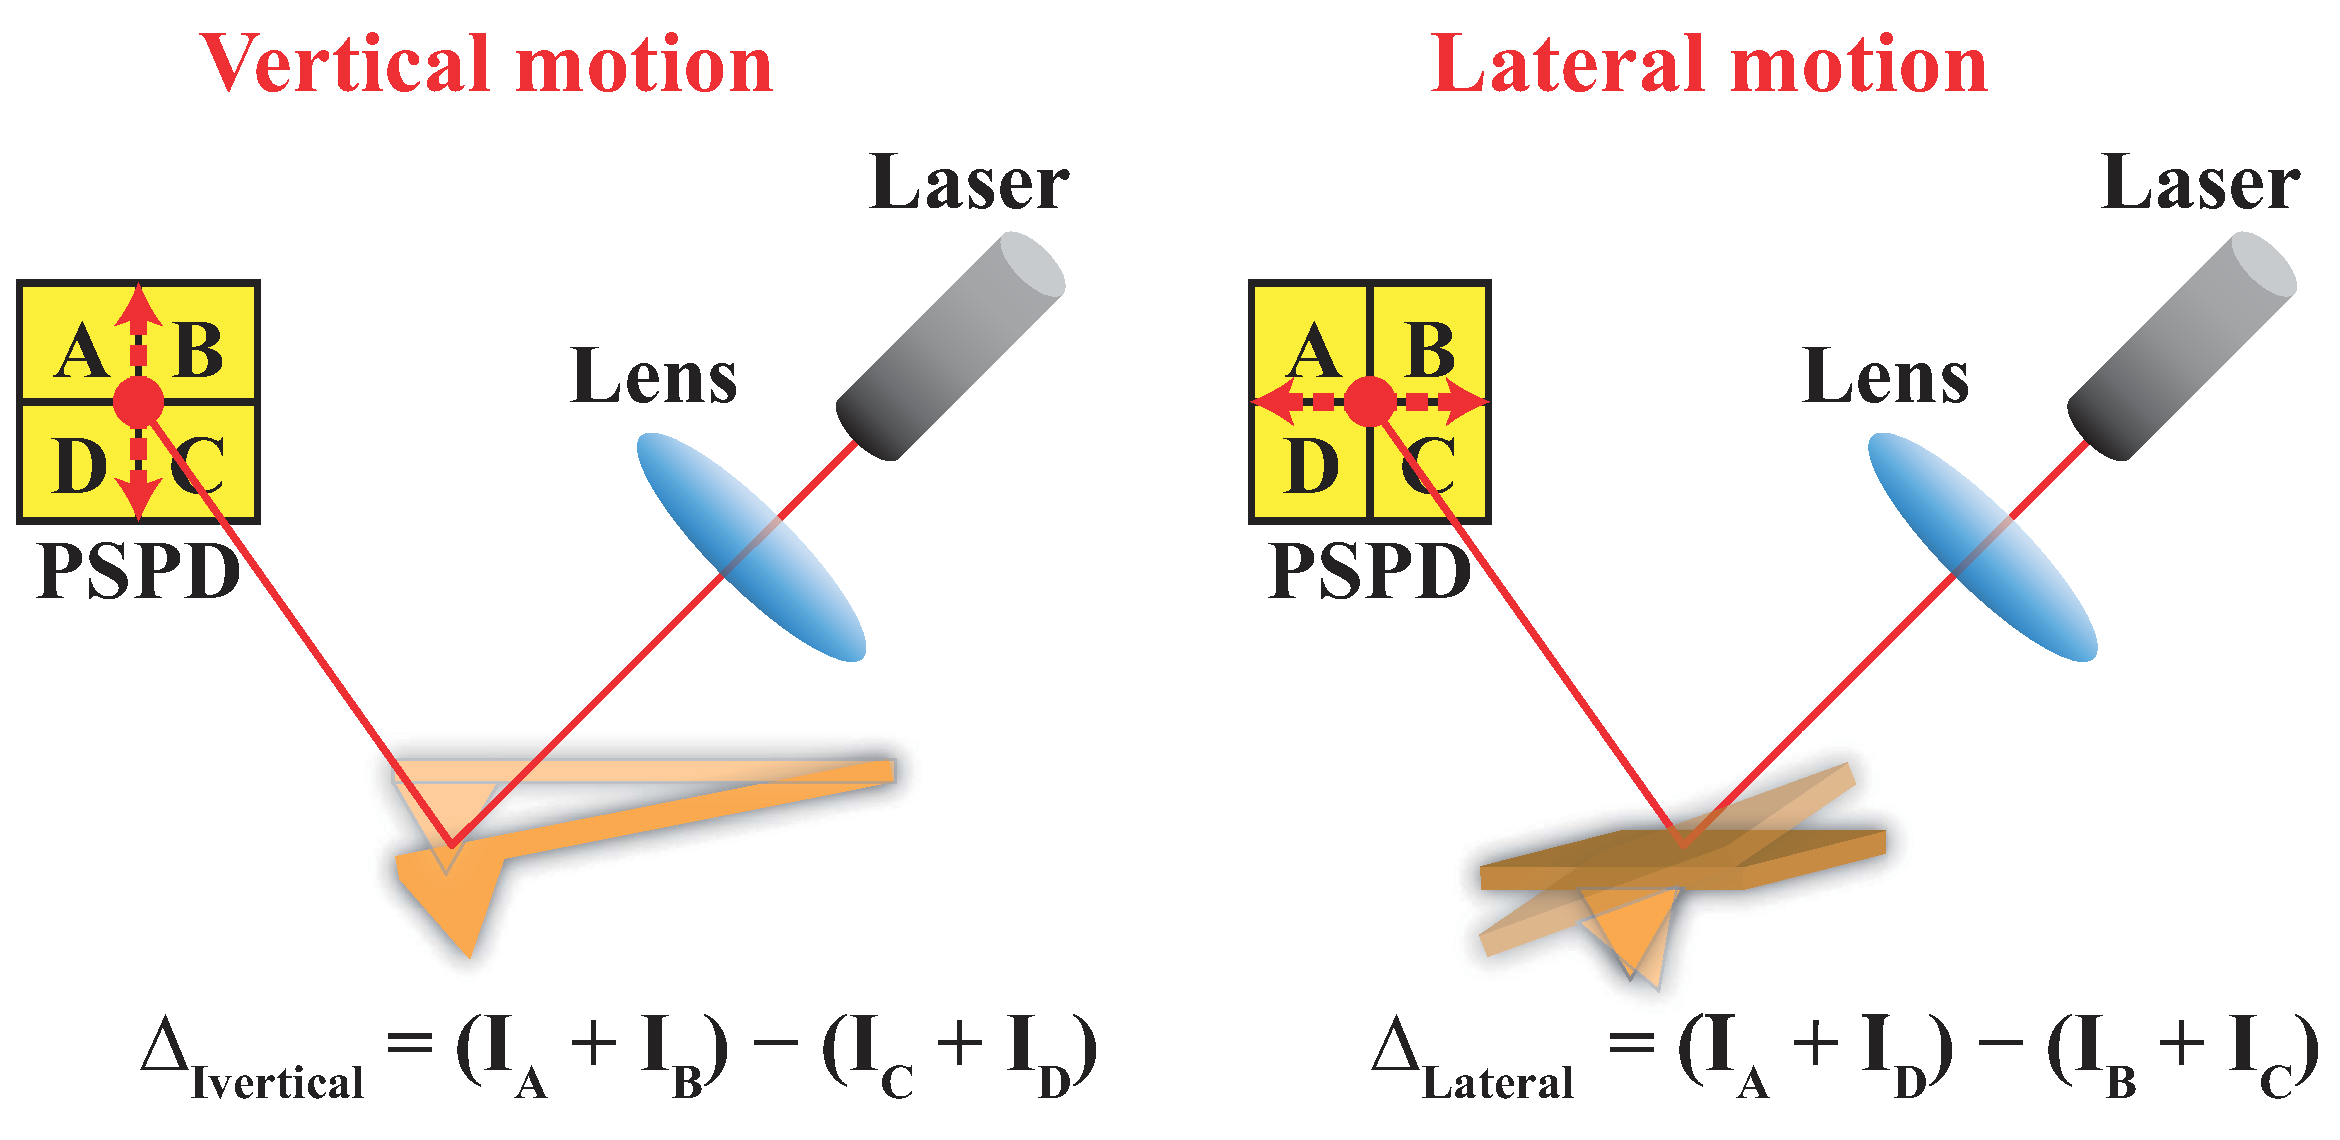
\includegraphics[scale=0.4]{EXP/afm2.eps}
\caption{\label{fig:afm2}Schematic of optical system for cantilever deflections detection.}
\end{figure}

The physical principle of the AFM operation is based on interaction between the probe tip and the specimen surface(Figure~\ref{fig:afm3}). When the cantilever approaches the specimen surface, Van der Waals forces start acting upon it . They are sufficiently far-ranging and are felt at the distance of a few tens of angstroms. Then at the distance of several angstroms repulsive force starts acting. In humid air a water layer is present on the specimen surface. The capillary force arises that holds the tip in contact with the surface and increases the minimum achievable interaction force. Electrostatic interaction between the probe and the sample may appear rather often. This can be both attraction and repulsion. Van der Waals attraction forces, capillary, electrostatic and repulsion forces at the point where the tip touches the sample and forces acting upon the tip from the deformed cantilever compensate each other in equilibrium. Based on the type and degree of this interaction the AFM modes can be broken down into contact and semi-contact(Figure~\ref{fig:afm3} ), which is a transition mode between the contact and non-contact modes.
\begin{figure}[htb]
\centering
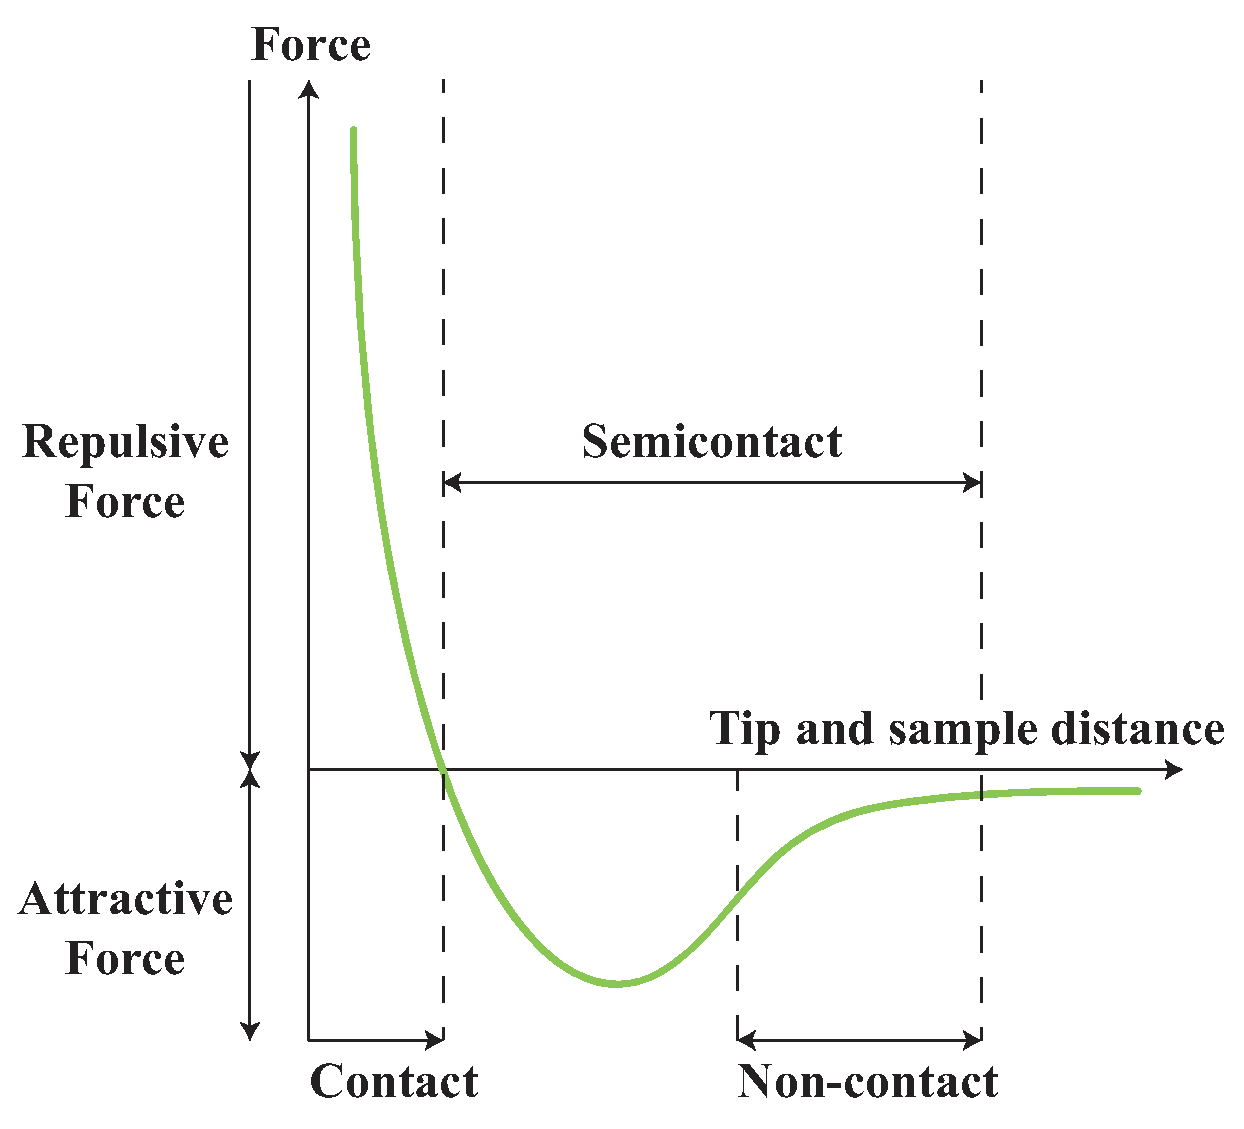
\includegraphics[scale=0.6]{EXP/afm3.eps}
\caption{\label{fig:afm3}Sketch of tip-sample forces.}
\end{figure}

\paragraph{Contact mode}

In contact mode of operation the cantilever deflection under scanning reflects repulsive force acting upon the tip. Repulsion force $\mathbf{F}$ acting upon the tip is related to the cantilever deflection value $\mathbf{x}$ under Hooke's law: $\mathbf{F}=-K \cdot  \mathbf{x}$, where $K$ is cantilever spring constant. The spring constant values for different cantilevers usually vary from 0.01 to several $\mathbf{N/m}$.

In our units the vertical cantilever deflection value is measured by means of the optical registration system and converted into electrical signal DFL (difference signal between the upper and lower halves of the PSPD) . In contact mode the DFL signal is used as a parameter characterizing the interaction force between the tip and the surface. There is a linear relationship between the DFL value and the force. In constant force mode of operation the deflection of the cantilever is maintained by the feedback circuitry on the preset value. So vertical displacement of the scanner under scanning reflects topography of sample under investigation.

Contact force microscopy is surface topography measurement in the contact mode.The microscope operation in the mode of maintaining constant interaction force between the tip and the surface sample, and is the base for measuring surface topography as well as for measuring local rigidity, local viscosity and local friction force. Constant force mode has some advantages and disadvantages. Main advantage of constant force mode is possible to measure with high resolution simultaneously with topography and some other characteristics, such as friction forces, spreading resistance etc. Constant force mode has also some disadvantages. Speed of scanning is restricted by the response time of feedback system. When exploring soft samples they can be destroyed by the scratching because the probe scanning tip is in direct contact with the surface. Therefore, under scanning soft unhomogeneous samples the local flexure of sample surface varies. As a result acquired topography of the sample can be proved distorted. Possible existence of substantial capillary forces imposed by a liquid adsorption layer can decrease the resolution.

\paragraph{Semi-contact mode}

The semi-contac mode can be characterized by some advantages in comparison with contact mode. First of all, in this mode the force of pressure of the cantilever onto the surface is less, that allows to work with softer materials such as polymers and bio-organics. The semi contact mode is also more sensitive to the interaction with the surface that gives a possibility to investigate some characteristics of the surface distribution of magnetic and electric domains, elasticity and viscosity of the surface. 

Widely used semi-contact mode has some disadvantage concerned with the usage of the feedback circuit. The scanning speed in semi-contact mode is restricted by the feedback circuit reaction time. This disadvantage can be overcome by the fact that under scanning new value of cantilever oscillation amplitude (and error signal) usually is achieved faster than preset value of the cantilever oscillation amplitude can be reached by the feedback system. Time of the reaching new value of the oscillation amplitude is determined by the oscillation period and Q-quality of the cantilever.
The feedback error signal, emerging when scanning in the semi-contact mode, contains some additional information about the topography. It can be utilized for achieving a more precise recovery of the relief. 

Additionally, similarly to the contact error mode, which can be considered as intermediate between the constant force mode and constant height mode, the feedback gain factor (i.e. the feedback processing speed) can be adjusted for the system to be able to trace subtle changes of the relief and to be too slow to trace the steep changes. Then, when the probe travels over minor irregularities, scanning will be carried out with an almost constant piezo scanner length. As a result, the slow changes of the relief will hardly show up on the images, and the steep changes will appear in high contrast. This may be helpful in finding minor irregularities on large areas against major sloping relief features. It must be noted that height of the minor irregularities must be less than amplitude of cantilever oscillation.

\section{Scanning electron microscopy}

The scanning electron microscope (SEM) is used for the observation of specimen surfaces~\cite{von1938elektronen}. When the specimen is irradiated with a fine electron beam, secondary electrons are emitted from the specimen surface. Topography of the surface can be observed by two-dimensional scanning of the electron probe over the surface and acquisition of an image from the detected secondary electrons. The concept schematic of commercial SEM (JEOL, JSM-6500F) is shown in Figure~\ref{fig:sem1}. The basic unit is composed of an electron optical system, a specimen stage, a secondary-electron detector, an image display unit, and an operation system. The electron optical system consists of an electron gun, a condenser lens and an objective lens to produce an electron probe, a scanning coil to scan the electron probe, and other components. The system inside of the microscope column are kept at vacuum.
\begin{figure}[htb]
\centering
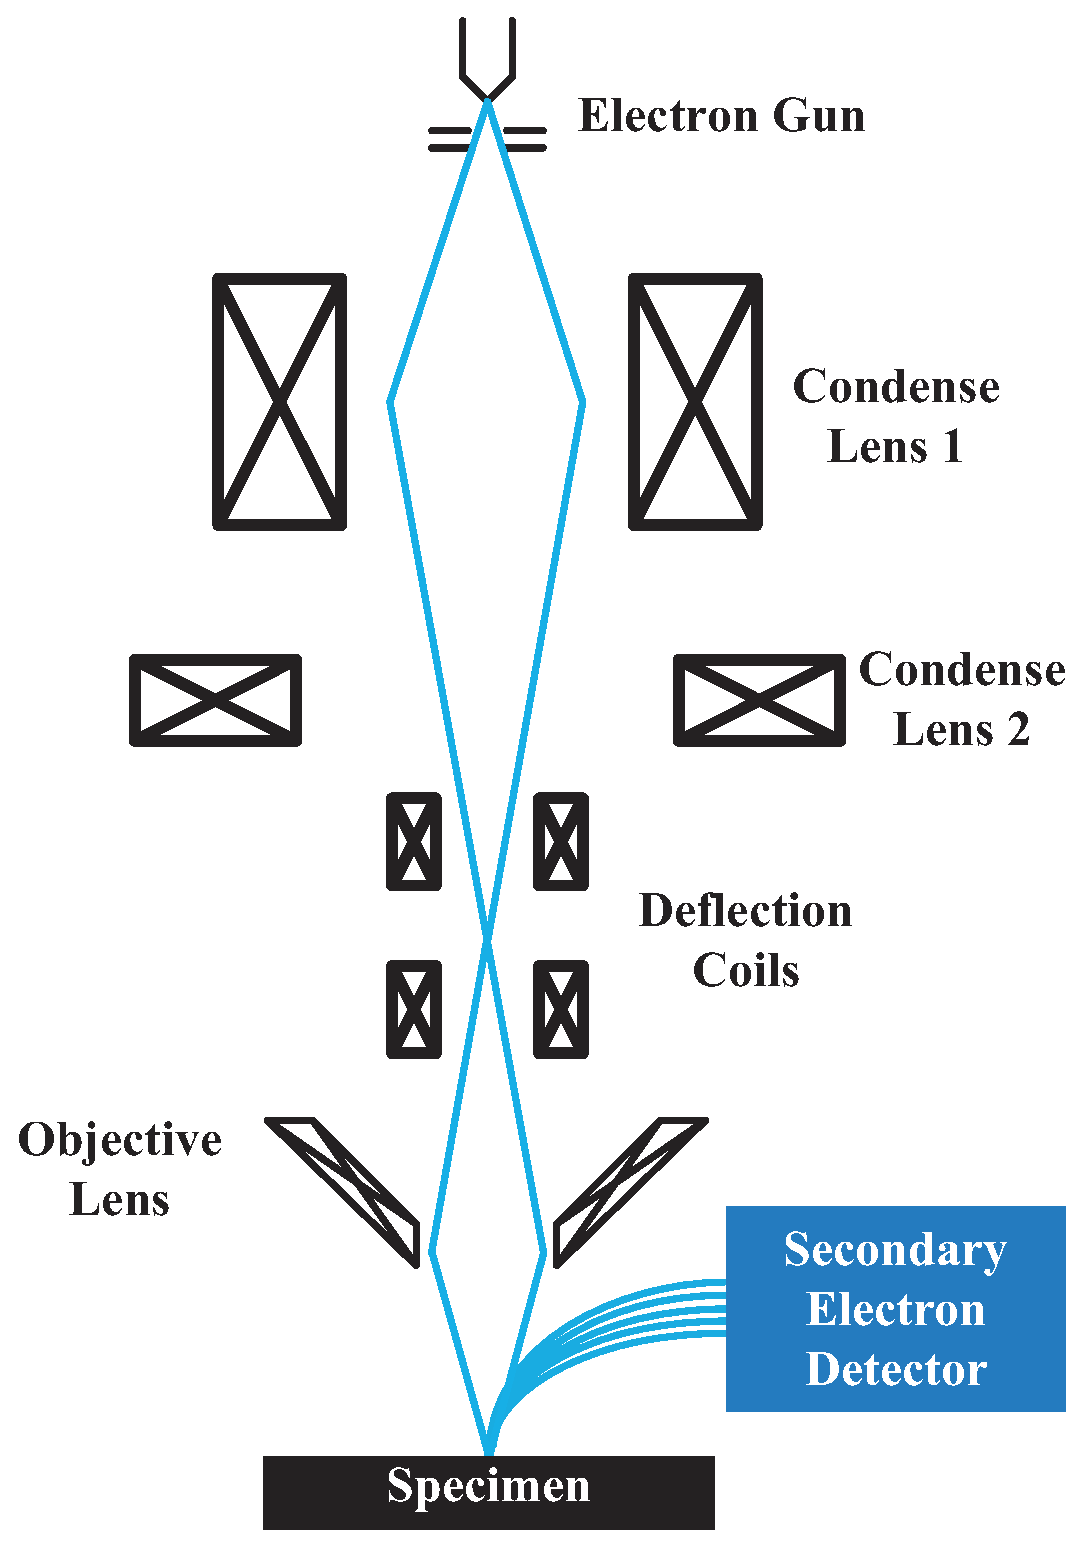
\includegraphics[scale=0.5]{EXP/SEM.eps}
\caption{\label{fig:sem1}Basic construction of a scanning electron microscopy.}
\end{figure}


The JSM-6500F utilizes a Schottky type field-emission (T-FE) gun for the electron source. The T-FE gun can constantly supply the surface of the cathode with zirconium oxide by heating the surface of cathode to 1800 K. For this reason, it can easily obtain stable and high probe current (range from several pA to 100 nA) compared with the traditional thermal emission electron gun and cold field-emission gun.

The magnetic condenser and objective lens system act to control the diameter of the beam as well as to focus the beam on the specimen due to a rotationally-symmetric magnetic field is formed when we pass a direct electric current through a coilwound electric wire in the magnetic lens. A pair of deflector coils, which between the condenser and objective lens, controlled by the scan generator, which are responsible for rastering that focused beam across the specimen surface. The size of the rastering pattern is under magnification control. The beam is rastered from left to right and top to bottom. There is a one-to-one correspondence between the rastering pattern on the specimen and the rastering pattern used to produce the image on the monitor. The resolution we choose to image at will obviously affect the number of pixels per row as well as the number of rows that constitute the scanned area.

The signal is generated from the specimen, and collected by the detector and subsequently processed to generate the image. That processing takes the intensity of the signal coming from a pixel on the specimen and converts it to a grayscale value of the corresponding monitor pixel. The monitor image is a two dimensional rastered pattern of grayscale values.

With the beam focused on the specimen surface, all we need to do to change magnification is to change the size of the rastered area on the specimen. The size of the monitor raster pattern is constant. Magnification will increase if we reduce the size of the area scanned on the specimen.

%\bibliographystyle{unsrt}
%\bibliography{thesisbib}
     \end{verbatim}
    最後記得在每個有附參考文獻的章節加上產生參考文獻的指令,即在\href{run:./introduction.tex}{introduction.tex}、\href{run:./THM.tex}{THM.tex}和\href{run:./EXP.tex}{EXP.tex}三個檔案裡最後啟動下面兩行指令
     \begin{verbatim}
%\bibliographystyle{unsrt} => \bibliographystyle{unsrt}
%\bibliography{thesisbib}  =>  \bibliography{thesisbib}
     \end{verbatim}
    而編譯時則需要對有附參考文獻的\href{run:./introduction.tex}{introduction.tex}、\href{run:./THM.tex}{THM.tex}和\href{run:./EXP.tex}{EXP.tex}各做一次BibTeX 編譯,編譯流程如下
    \begin{enumerate}[topsep=0pt, itemsep=0pt, label=\arabic{*}.]
    \item \texttt{xelatex thesis}\\ 對thesis.tex進行第一次XeLaTeX編譯,產生thesis.pdf及其他檔案
    \item \texttt{bibtex introduction}\\ 對introduction.tex進行BibTeX編譯,產生bbl檔以及blg檔
    \item \texttt{bibtex THM}\\ 對THM.tex進行BibTeX編譯,產生bbl檔以及blg檔
    \item \texttt{bibtex EXP}\\ 對EXP.tex進行BibTeX編譯,產生bbl檔以及blg檔
    \item \texttt{xelatex thesis}\\ 對thesis.tex進行第二次XeLaTeX編譯,產生目錄、圖表連結及參考文獻
    \item \texttt{xelatex thesis}\\ 對thesis.tex進行第三次XeLaTeX編譯,產生參考文獻連結,完成編譯\\
\end{enumerate} 
\item 補充說明與注意事項:
\begin{enumerate}[topsep=0pt, itemsep=0pt, label=$\bullet$]
    \item 口試委員會審定書:\\
    請到台大圖書館網頁的\href{http://etds.lib.ntu.edu.tw/etdsystem/submit/submitLogin}{電子論文服務}下載\href{http://gra103.aca.ntu.edu.tw/gra2007/gra/tienn/\%E5\%AD\%B8\%E4\%BD\%8D\%E8\%80\%83\%E8\%A9\%A6\%E8\%A1\%A8\%E5\%86\%8A/THESISSAMPLE.DOC}{論文格式範本},並修改成正確的格式,也可到此範本所在資料夾的\href{run:./cert.doc}{cert.doc}修改。當然你也可以利用LaTeX來編輯,你只要填好\href{run:./ntuvars.tex}{ntuvars.tex}檔的資料,並去除在thesis.tex裡下面這行的註解符號\texttt{\%} 
    \begin{verbatim}
%\makecertification
    \end{verbatim}
    編譯完後就可以產生審定書格式。口試通過後,請把已經簽名的審定書掃描成pdf檔,再取代原本的\href{run:./cert.pdf}{cert.pdf},即可放上已簽名的審定書。處理審定書出現的指令在thesis.tex裡 
    \begin{verbatim}
%----------- generate the certification ...
%\makecertification
%----------- includepdf by using package ...
\addcontentsline{toc}{chapter}{口試委員會審定書}
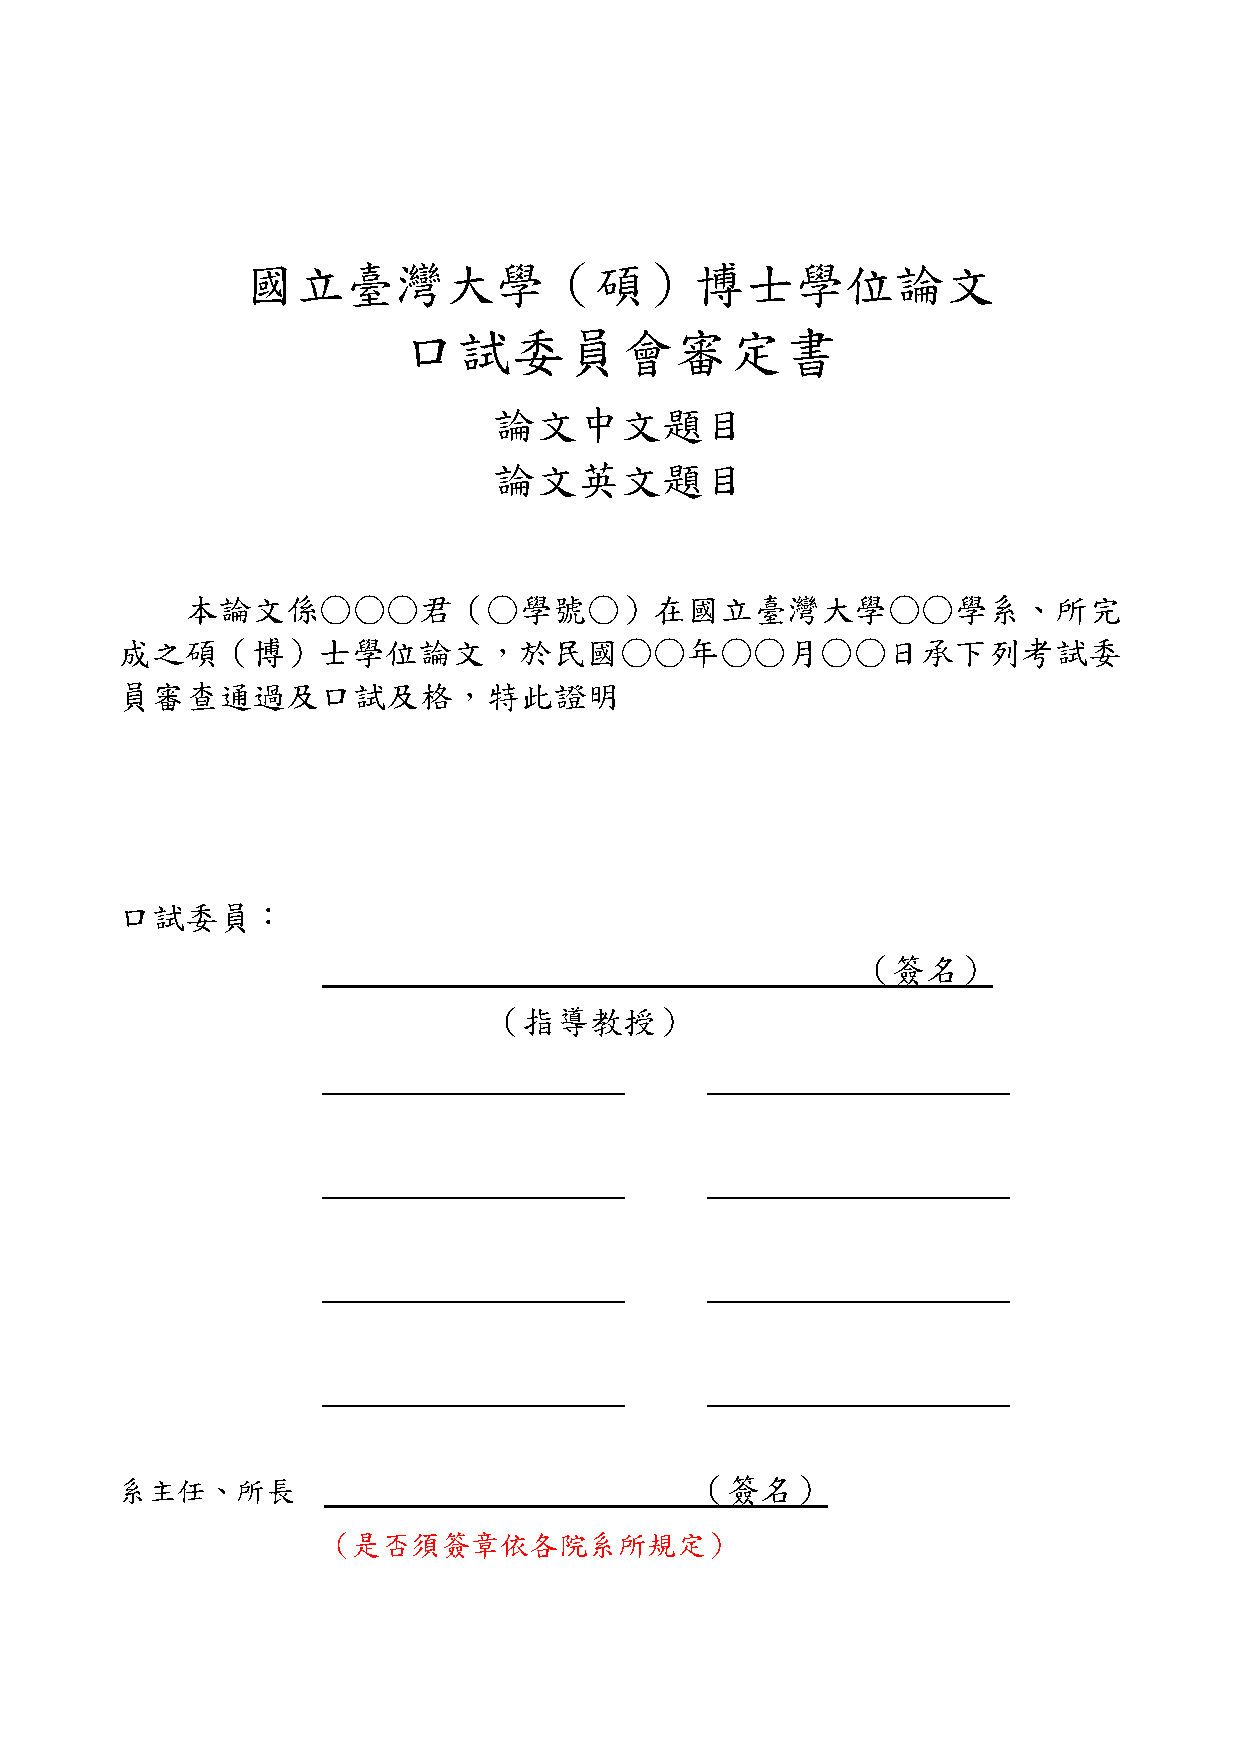
\includepdf[pages={1}]{cert.pdf}
    \end{verbatim}
    \item 浮水印:\\
    資料夾已經附上浮水印檔案了,若學校有更改,到請到台大圖書館網頁的\href{http://etds.lib.ntu.edu.tw/etdsystem/submit/submitLogin}{電子論文服務}下載\href{http://etds.lib.ntu.edu.tw/files/watermark.pdf}{pdf格式的浮水印}到此範本所在資料夾。若要開啟關閉浮水印功能,即自行刪去或加上下面位於thesis.tex指令的註解符號\texttt{\%}
    \begin{verbatim}
%\CenterWallPaper{0.365}{watermark.pdf}
    \end{verbatim}
    \item 單面印刷與雙面印刷:\\
    此範本為單面印刷,若論文頁數超過80頁,依規定需要用雙面印刷,此時只需把thesis.tex裡的
    \begin{verbatim}
\documentclass[a4paper, 12pt, oneside]{book}
改成
\documentclass[a4paper, 12pt, twoside]{book}
    \end{verbatim}
    \item \XeTeX\ :\\
    此範本中文字體使用\XeTeX\ 轉換,細節請參考\href{http://www.hitripod.com/blog/}{Hitripod}寫的\href{http://www.hitripod.com/blog/2011/04/xetex-chinese-font-cjk-latex/}{ 
XeTeX:解決 LaTeX 惱人的中文字型問題}。
    \end{enumerate} 
    \end{enumerate} 

%----------- Have a fractal fern? -----------
%\begin{pspicture}
%\psFern[scale=30,maxIter=100000,linecolor=Green]
%\end{pspicture}

 \end{acknowledgementsCH}